\documentclass[letterpaper, 10 pt, conference]{ieeeconf}  % Comment this line out if you need a4paper

%\documentclass[a4paper, 10pt, conference]{ieeeconf}      % Use this line for a4 paper

\IEEEoverridecommandlockouts                              % This command is only needed if
                                                          % you want to use the \thanks command

\overrideIEEEmargins

% \usepackage[pdftex]{graphicx}
\usepackage{array}
\usepackage{fancyhdr}
\usepackage{graphicx}
\usepackage{amsfonts}
\usepackage{amssymb}
\usepackage{amsmath}
\usepackage{verbatim}
\usepackage{color}
% \usepackage{marvosym}

\usepackage{hyperref}
\hypersetup{
%    bookmarks=true,         % show bookmarks bar?
%    unicode=false,          % non-Latin characters in Acrobat's bookmarks
%    pdftoolbar=true,        % show Acrobat's toolbar?
%    pdfmenubar=true,        % show Acrobat's menu?
    pdffitwindow=false,     % window fit to page when opened
    pdfstartview={FitH},    % fits the width of the page to the window
%    pdftitle={My title},    % title
%    pdfauthor={Author},     % author
%    pdfsubject={Subject},   % subject of the document
%    pdfcreator={Creator},   % creator of the document
%    pdfproducer={Producer}, % producer of the document
%    pdfkeywords={keyword1} {key2} {key3}, % list of keywords
    pdfnewwindow=true,      % links in new window
    colorlinks=true,       % false: boxed links; true: colored links
    linkcolor=red,          % color of internal links
    citecolor=green,        % color of links to bibliography
    filecolor=magenta,      % color of file links
    urlcolor=cyan           % color of external links
}
%\usepackage{pdfpages} % para incluir pdfs

%\usepackage[hyphens]{url}

\usepackage{cite}

% \usepackage{subcaption} %  for subfigures environments

\usepackage{listings}
\usepackage{hyperref} %allow inline hyperlinks
\usepackage[nolist,nohyperlinks]{acronym}

\usepackage{amsmath}
\usepackage{booktabs}
\usepackage{multicol}
\usepackage{multirow}
% \usepackage{todonotes}

% note that cleverref must be loaded after hyperref
\usepackage[capitalise]{cleveref}

%get rid of ugly red boxes around links
\usepackage{color} % let's have some color!
\usepackage{xcolor}
\hypersetup{
    colorlinks=true,
    linkcolor={red!70!green},  %Color of internal links
    citecolor={blue!50!green}, %Color of citations
    urlcolor={blue!80!black}   %Color for external hyperlinks
}

\newcommand{\Munzir}[1]{{\color{red}{#1}}}
\newcommand{\ie}{\textit{i}.\textit{e}., }

% Stop showing all the authors and follow the IEEE convention of, if there are
% more than six authors for a reference, only show first author and et al in
% refs list
% From https://tex.stackexchange.com/a/164513
% These lines are in the bib file now
% @IEEEtranBSTCTL{IEEEexample:BSTcontrol,
% CTLuse_forced_etal = "yes",
% CTLmax_names_forced_etal = "6",
% CTLnames_show_etal = "1"}

% Typeset units consistently
\usepackage[per-mode=symbol]{siunitx}

\newcommand{\fixme}[1]{\textcolor{red}{\textbf{fix me:} #1}}
\newcommand{\Bogdan}[1]{\textcolor{red}{\textbf{Bogdan:} #1}}
\newcommand{\Nathan}[1]{\textcolor{red}{\textbf{Nathan:} #1}}


%%%%%%%%%%%%%%%%%%%%%%%%%%%%%%%%% Packages I copied from PhD Proposal%%%%%%%%%%%%%%%%%%%%%%%%%%%%%%%%%%%%%%%%%%
%%%%%%%%%%%%%%%%%%%%%%%%%%%%%%%%%%%%%%%%%%%%%%%%%%%%%%%%%%%%%%%%%%%%%%%%%%%%%%%%%%%%%%%%%%%%%%%%%%%%%%%%%%%%%%%
%%%%%%%%%%%%%%%%%%%%%%%%%%%%%%%%%%%%%%%%%%%%%%%%%%%%%%%%%%%%%%%%%%%%%%%%%%%%%%%%%%%%%%%%%%%%%%%%%%%%%%%%%%%%%%%
\usepackage{algorithm,algorithmic}
\newenvironment{conditions}
  {\par\vspace{\abovedisplayskip}\noindent\begin{tabular}{>{$}l<{$} @{${}={}$} l}}
  {\end{tabular}\par\vspace{\belowdisplayskip}}



\DeclareGraphicsExtensions{.pdf,.jpeg,.png}

% correct bad hyphenation here
%\hyphenation{op-tical net-works semi-conduc-tor MATLAB}

\begin{document}
\frenchspacing

\title{\LARGE \bf Online Center of Mass Estimation for a \\Humanoid Wheeled Inverted Pendulum Robot}

\author{Munzir Zafar$^*$, Akash Patel$^*$, Bogdan Vlahov, Nathaniel Glaser, Sergio Aguilera, Seth Hutchinson
%\author{Albert Author$^{1}$ and Bernard D. Researcher$^{2}$% <-this % stops a space
%\thanks{*This work was not supported by any organization}% <-this % stops a space
\thanks{$^{*}$Joint First Authors}%
\thanks{Munzir Zafar, Akash Patel, Bogdan Vlahov, Nathaniel Glaser, Sergio Aguilera and Seth Hutchinson are with the Institute of Robotics and Intelligent Machines at the Georgia Institute of Technology, Atlanta, GA, 30332, USA. email: {\tt\small mzafar7@gatech.edu, apatel435@gatech.edu, bvlahov3@gatech.edu, nglaser@gatech.edu, sfaguile@gatech.edu, seth@gatech.edu}}%
}


\begin{acronym}
\acro{CoM}{Center of Mass}
\acroplural{CoM}[CoMs]{Center of Masses}
\acro{WIP}{Wheeled Inverted Pendulum}
\acro{DoF}{Degree of Freedom}
\acroplural{DoF}[DoFs]{Degrees of Freedom}
\acro{RRT}{Randomly-Exploring Random Trees}
\acro{ESO}{Extended State Observer}
\acro{ADRC}{Active Disturbance Rejection Control}
\acro{PID}{Proportional-Integral-Derivative}
\acro{BLR}{Bayesian Linear Regression}
\acro{LQR}{Linear Quadratic Regulator}
\acro{DART}{Dynamic Animation and Robotics Toolkit}
\end{acronym}


\maketitle
\thispagestyle{empty}
\pagestyle{empty}
% \Bogdan{General Notes: The paper is not consistent throughout. Some large problems I see are in the organization of the learning sections and uncertainty in the number of \acsp{DoF} we have. We also are probably repeating content again in the learning sections. If you guys want to meet up today, let me know}
%%%%%%%%%%%%%%%%%%%%%%%%%%%%%%%%%%%%%%%%%%%%%%%%%%%%%%%%%%%%%%%%%%%%%%%%%%%%%%%%
%%%%%%%%%%%%%%%%%%%%%%%%%%%%%%%%%%%%%%%%%%%%%%%%%%%%%%%%%%%%%%%%%%%%%%%%%%%%%%%%
%%%%%%%%%%%%%%%%%%%%%%%%%%%%%%%%%%%%%%%%%%%%%%%%%%%%%%%%%%%%%%%%%%%%%%%%%%%%%%%%
\begin{abstract}

We present a novel application of robust control and online learning for the balancing of a n \ac{DoF}, \ac{WIP} humanoid robot.
Our technique condenses the inaccuracies of a mass model into a \ac{CoM} error, balances despite this error, and uses online learning to update the mass model for a better \ac{CoM} estimate.
Using a simulated model of our robot, we meta-learn a set of excitory joint poses that makes our gradient descent algorithm quickly converge to an accurate \ac{CoM} estimate.
% we evolve between these poses using \ac{RRT} with simulated collision detection;
%and we use gradient descent to improve the \ac{CoM} estimate.
This simulated pipeline executes in a fully online fashion, using active disturbance rejection to address the mass errors that result from a steadily evolving mass model.
Experiments were performed on a 19 \ac{DoF} \ac{WIP}, in which we manually acquired the data for the learned set of poses and show that the mass model produced by a gradient descent produces a \ac{CoM} estimate that improves overall control and efficiency.
This work contributes to a greater corpus of whole body control on the Golem Krang humanoid robot.

\end{abstract}

%%%%%%%%%%%%%%%%%%%%%%%%%%%%%%%%%%%%%%%%%%%%%%%%%%%%%%%%%%%%%%%%%%%%%%%%%%%%%%%%
%%%%%%%%%%%%%%%%%%%%%%%%%%%%%%%%%%%%%%%%%%%%%%%%%%%%%%%%%%%%%%%%%%%%%%%%%%%%%%%%
%%%%%%%%%%%%%%%%%%%%%%%%%%%%%%%%%%%%%%%%%%%%%%%%%%%%%%%%%%%%%%%%%%%%%%%%%%%%%%%%
\section{Introduction}
\label{sec:intro}
\acresetall{}
%\fixme{Switch to the guideline discussed. Start with a description of the difference between theory and practice and discuss the role of disturbance rejection as a bridge between the two. Then go on to show an example of this method (Online \ac{CoM})}

Combining the maneuverability of a two-wheeled mobile platform and the dexterity of robotic arms, humanoid \ac{WIP} robots present novel challenges to the robotics research community.
% Extensive prior research exists for \ac{WIP} balancing and robot arm manipulation \Bogdan{I think we need citations for WIP and Robot arm Manipulation here}, individually; however, when combined, the resulting system poses challenges more interesting than the sum of its parts.  In naive implementations of humanoid \ac{WIP} robots, balancing tasks are decoupled from manipulation tasks.  This decoupling is simple to implement, but it is unnatural for truly human-like motion.
%Keeping the balance of the WIP as the one presented in Fig.~\ref{fig: system1} is fundamental to keep the robot safe and accomplish its objectives. Whatever the robot is doing, the low level controllers will always be working to keep the balance of the robot.
% Stabilizing control of \ac{WIP} humanoid robots has been an active research topic as it combines the dexterity of robotic arms and the maneuverability of the \acp{WIP}.
Humanoid robot stabilization is fundamental to keep the robot safe and for the robot to accomplish higher-level objectives.
Furthermore, keeping a \ac{WIP}, such as the one presented in Fig.~\ref{fig: system1}, balanced is a fundamental task in which the controller needs to be constantly working and thus should be energy efficient \cite{Bature2014}.
Stabilization is usually accomplished through the control of a simplified two \ac{DoF} model which summarizes the \ac{CoM} of all the joints into one as shown in Fig~\ref{fig: system}. This simplification is usually done for both \ac{WIP} humanoid robots \cite{Zafar2016,canete2012disturbance, takei2009baggage}, as well as for legged humanoids \cite{Carpentier2016, Muscolo2011, Kudruss2015}.
All frameworks presented to stabilize \ac{WIP} robots consider that the mass and \ac{CoM} for each of the joints is accurately known \cite{SangJoo2007,Sihite2018,Pajon2017} to compute the simplified two \ac{DoF}  WIP model. However, the mass and real location of the \ac{CoM} is difficult to obtain, as robot systems can be complex and they might change throughout time. The discrepancy in the parameters of the robot affects the controller's performance, diminishing the robot's dexterity and increasing the power consumption.

Regarding these uncertainties in the model, one common control methodology uses the Modern Control Paradigm \cite{Gao2006} which focuses on the modeling of the system as, $\ddot{y} = f(y,\dot{y},w,t) + bu$, where $y$ is the position output and $w$ is an unknown input force. Once the system is modeled, it is approximated to a linear, time-invariant and disturbance-free model, to design a control law. This approach relies on the model approximation $\bar{f}(\dot{y},y)$ to be ``close enough'' to the real model in the neighborhood of the operation point. In \cite{Gao2006} and later in \cite{canete2012disturbance}, \acp{ESO} are used to estimate the modeled uncertainties and improve the control of the systems. The approach used collapses all the uncertainties and external forces under one element which is later eliminated through feedback control.  From an online learning approach, commonly used models rely on the knowledge and accuracy of the \ac{CoM} \cite{Luo2012,Chen2017,Yang2016}. Very few have worked on model parameter estimation such as \cite{Kim2016,Jamone2014}, but focus more on the estimation of external parameters such as terrain coefficient or external forces than on the robot itself. Finally, recent research involving mobile manipulators has focused on the use of \ac{ADRC} \cite{Jiang2016,Ruan2014,Wei2017} to control systems which use external uncertainties to conduct feedback control.

\begin{figure}[t]
	\centering
	%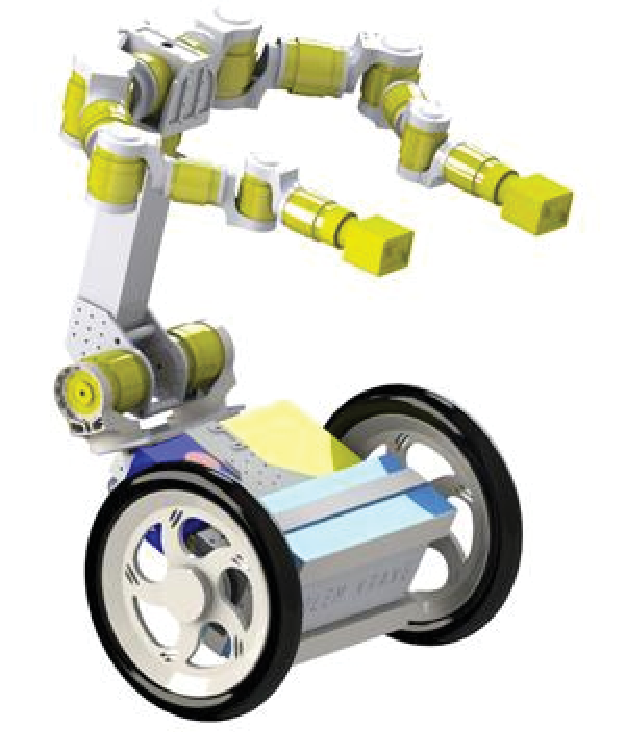
\includegraphics[width=0.4\columnwidth]{figs/System1.pdf}
	\includegraphics[width=0.4\columnwidth, clip]{figs/System1.eps}
	\vspace{-0.5\baselineskip}
   \caption{Full Body of our WIP Humanoid.}
   \label{fig: system1}
\end{figure}

Our approach improves our model parameter estimation using the knowledge of the \ac{ESO} through online learning.
%We propose a methodology to improve our model and control through online learning scheme using \ac{ESO}.
The goal of this framework is to create models that are improved upon by real-world systems and data. %The main idea of our methodology is,
Given a model of our system, we want to improve the values of the parameters by measuring the disturbances of the system when it is not subject to external forces. Then, as the robot changes its joints position, we are able to update our parameters in an online fashion.
To accomplish this task, we propose the following methodology. Given an initial estimation of the parameters of our model $\beta_0$, we use \ac{ADRC} \cite{Gao2006} to estimate the error between the parameters estimated \ac{CoM} and the real one for different joint configurations. This error is used to update our knowledge of the model parameters through gradient descent. We show that this methodology works, but it might take numerous positions to converge. Thus, we propose a meta-learning algorithm to find the poses which induce the largest gradient step for gradient descent.
The main contributions of this works are: \textit{i)} a novel use of the \ac{ESO} and \ac{ADRC} to estimate the error in the model parameters; \textit{ii)} an online learning algorithm to update and improve our model parameters; \textit{iii)} a meta-learning framework to improve the speed and accuracy of our learning algorithm; \textit{iv)} and  preliminary results on a real robot with 19 \ac{DoF} that show the improvement of the system's performance.

This paper is organized as follows. Section \ref{sec:method} presents the \ac{WIP} robot and the methodology, as well as discusses the learning, meta-learning, and \ac{ADRC} techniques. Sections \ref{sec:experimental_design} and \ref{subsec:results} describe and present the different simulations and experiments. Finally, section \ref{sec:conclusion} presents the conclusions of our work.

\section{Methodology}
\label{sec:method}

The goal of the proposed approach is to improve the \ac{CoM} estimate of a \ac{WIP} Humanoid. A \ac{WIP} Humanoid is a highly redundant manipulator mounted on a differential wheeled drive able to dynamically balance itself in an inverted pendulum configuration (Fig \ref{fig: system}). A good estimate of the \ac{CoM} is important for any approach to control dynamically balancing humanoids. This is because the balancing task requires the \ac{CoM}'s ground projection to always lie in the support polygon. The support polygon of a WIP is a rectangle on width equal to the distance between the wheels and a small length given by the compression of the wheels against the ground. This support polygon is very thin, hence is important to decreasing the room for errors in \ac{CoM} estimates compared to, say, bipedal humanoids where support polygons are much larger.

Let us define frame $0$ as the frame where the origin  is located at the midpoint between the wheels with its $x$-axis always along the heading direction and $z$-axis always vertical. We are interested in the coordinates of the \ac{CoM} of the body in this frame. Specifically, we want the $x$-coordinate of body \ac{CoM} in this frame to be zero in order to balance the robot. Homogeneous coordinates of body CoM in frame $0$ are given by
\begin{align}
    X_{com}(q) \!= \!\begin{bmatrix} x_{com}(q) \\ y_{com}(q) \\ z_{com}(q) \\ 1 \end{bmatrix} &\!= \! \frac{\sum_{i}^{L} m_i X_i^0(q)}{\sum_{i}^{L} m_i} \!= \! \frac{\sum_{i}^{L} m_i {T}_{i}^{0}(q)X_i^i}{\sum_{i}^{L} m_i} \nonumber
\end{align}
where we are interested in the $x$ component of the CoM
\begin{align}
    x_{com}(q) &= \phi(q)^\top \beta \label{eq:xcom}
\end{align}
and the variables are described in Table~\ref{tab:Variables}.
% \begin{conditions}
%     L & number of links in the body \\
%     q & $\begin{bmatrix} q_1 & ... & q_L \end{bmatrix}^\top$ position of all joints in the body \\
%     m_i & mass of link $i$ \\
%     X_i^0(q) & is CoM of link $i$ expressed in frame $0$ \\
%     X_i^i & $\begin{bmatrix} x_i & y_i & z_i & 1 \end{bmatrix}^\top$ local CoM of local frame $i$ \\
%     T_{i}^{0}(q) & transformation from frame $i$ to frame $0$ \\
%     \beta & $\begin{bmatrix} m_1X_1^{1\;\top} & ... & m_L X_L^{L\;\top} \end{bmatrix}^\top \in \mathcal{R}^{4L}$ \\
%     \phi(q) & $\begin{bmatrix} \phi_1(q) & ... & \phi_{4L}(q) \end{bmatrix}$ \\
%     & feature vector of known geometric functions of $q$ \\
% \end{conditions}
\begin{table}[b]
    \centering
    \caption{\label{tab:Variables}System variables.}
    \begin{tabular}{c|p{0.79\columnwidth}}
    Variable & Description \\
    \hline
    $L$ & number of links in the body \\
    % \hline
    $q$ & $\begin{bmatrix} q_1 & ... & q_L \end{bmatrix}^\top$ position of all joints in the body \\
    % \hline
    $m_i$ & mass of link $i$ \\
    % \hline
    $X_i^0(q)$ & is CoM of link $i$ expressed in frame $0$ \\
    % \hline
    $X_i^i$ & $\begin{bmatrix} x_i & y_i & z_i & 1 \end{bmatrix}^\top$ local CoM of local frame $i$ \\
    % \hline
    $T_{i}^{0}(q)$ & transformation from frame $i$ to frame $0$ \\
    % \hline
    $\beta$ & $\begin{bmatrix} m_1X_1^{1\;\top} & ... & m_L X_L^{L\;\top} \end{bmatrix}^\top \in \mathcal{R}^{4L}$ \\
    % \hline
    $\phi(q)$ & $\begin{bmatrix} \phi_1(q) & ... & \phi_{4L}(q) \end{bmatrix}^\top$ feature vector of known geometric functions of $q$ \\
    % \hline
    \end{tabular}
\end{table}

\begin{figure}[htb]
	\centering
	%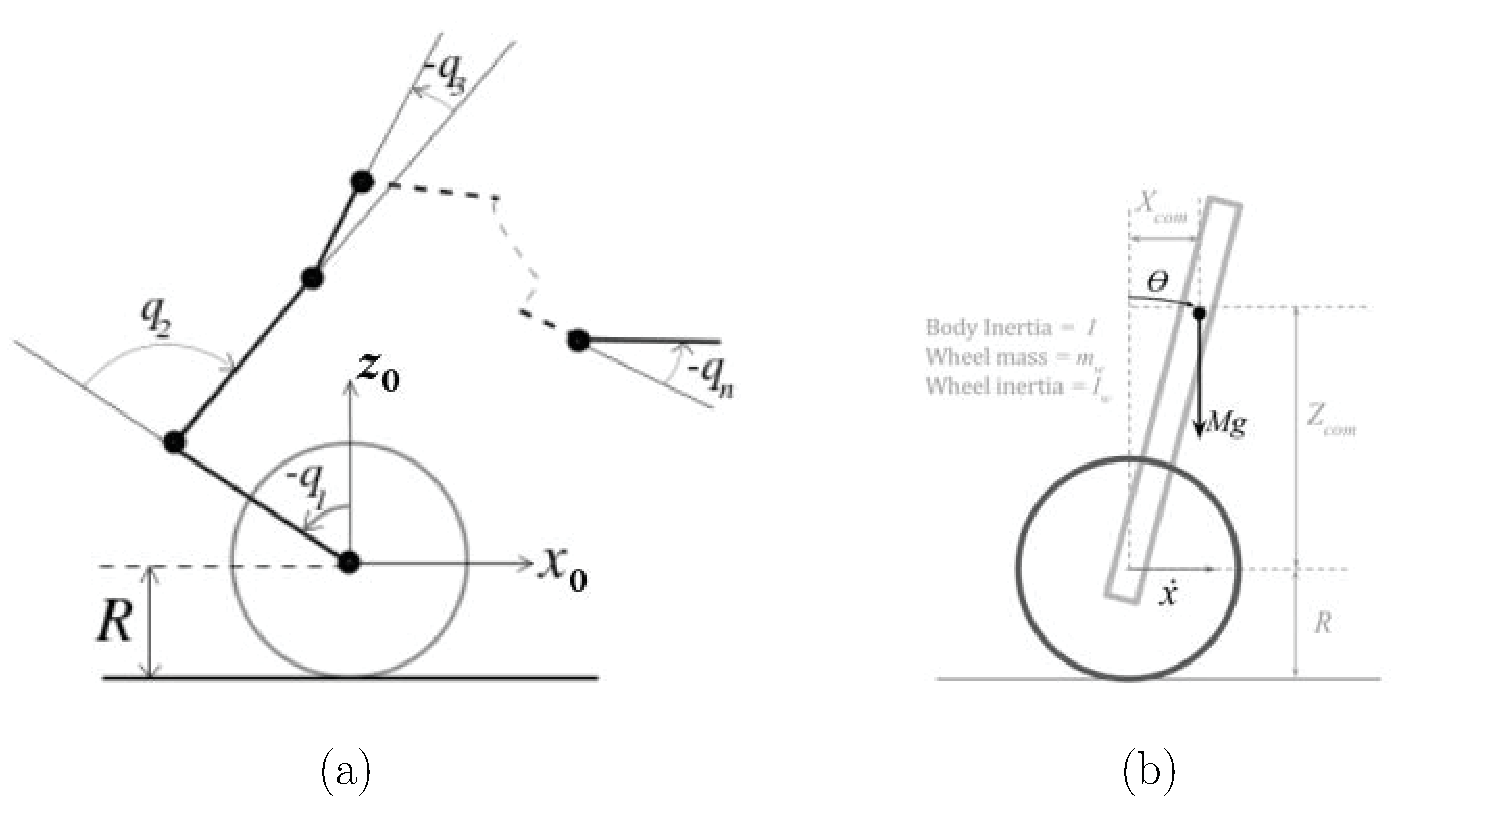
\includegraphics[width=0.9\columnwidth]{figs/System2.pdf}
	\includegraphics[width=0.9\columnwidth]{figs/System2.eps}
    \vspace{-.5\baselineskip}
    \caption{Full Body of a typical WIP Humanoid with $n$ links (a) 2D Simplified Model (b)}
    \label{fig: system}
\end{figure}

$\beta$ is the set of unknown parameters comprising mass and mass times \ac{CoM} of individual links in the body. This choice of parameters is such that the parameters appear linearly in the model. Treating \ac{CoM} values independently from masses would make the model quadratic in parameters. Improving the estimate of the body's \ac{CoM} entails improving our knowledge of $\beta$. One way to achieve this is to disassemble the robot into individual links and perform physical measurements for mass and \ac{CoM} of each link. This is tedious and hence undesirable. However, the fact that the \ac{CoM} model is linear in $\beta$ allows us to use linear regression or gradient descent to improve our model parameter estimates. We choose gradient descent because of its ability to enforce physical consistency constraints. For one, it converges to $\beta$ values in the neighborhood of the initial $\beta$ which are more likely to be physically consistent as opposed to linear regression which might learn solutions that fit the data but are physically nonsensical. Secondly, constraints such as total body mass can be explicitly enforced in the learning process through the use of Lagrange multipliers. The details of this appear in \cref{subsec: learning}.

These learning techniques rely on our ability to collect data for poses $q$ and corresponding values of outputs $x_{com}(q)$. The simplest way to collect this data is to make use of the fact that in the ideal case, $x_{com}(q) = 0$ when the robot is in a balanced state. Assuming that all joints in the body  shown in Fig. 1b can be locked at a specific pose $\{$ $q_2$, $...$, $q_L$ $\}$, there exists a position for $q_1$ (the base link) that can balance the robot. We can collect data offline by manually moving $q_1$ such that the robot is in a balanced state. However, this is again tedious; performing the same job online would avoid this labor. To this end, we utilize \ac{ADRC} \cite{canete2012disturbance} to balance the robot despite a bad estimate of body \ac{CoM}, the details of which appear in \cref{subsec: online}. One may ask: Why the need to improve  the \ac{CoM} model if there already exists a controller that is able to stabilize the robot despite a bad \ac{CoM} estimate? The answer to this is twofold: Firstly, \ac{ADRC} achieves balancing but is inefficient, i.e. it takes more time and aggressive control inputs to stabilize a bad estimate of \ac{CoM}. Secondly, \ac{ADRC} works only when controlling a single rigid link on wheels which is the case when body joints are locked. If however the joints are unlocked, more complex controllers are needed that rely on an accurate estimate of the \ac{CoM}.

We have so far discussed how to obtain the value of $x_{com}(q)$ at any give pose $q$. It is important to determine what poses at which we should collect this data. This is because with a highly redundant system, the configuration space is too large and relying on arbitrary poses may make the learning process inefficient and time-consuming. We choose poses such that every next pose causes the largest average gradient descent step over a large set of randomly chosen erroneous $\beta$ estimates. This is discussed in \cref{subsec: learning}.

% Finally, we lay out the method of planning trajectories that avoid self-collision and collision with the ground as the robot moves from pose to pose for data collection while balancing. For this purpose, we make use of constrained RRT. This is discussed in \ref{subsec: plan}.

\subsection{Learning Algorithm} \label{subsec: learning}

For the learning algorithm, we make use of gradient descent. The objective function to be minimized is determined based on the fact the $x$-component of CoM should be zero in a balanced pose. In order to make the cost function locally convex with respect to $\beta$, we aim to minimize the square of the $x$-component of CoM.
\begin{align}
    J(\beta) &= \tfrac{1}{2} \left[ x_{com}(q; \beta) \right]^2 \nonumber \\
    &= \tfrac{1}{2} \beta^\top \phi(q) \phi(q)^\top \beta
\end{align}
where we have made use of the definition of $x_{com}$ in \eqref{eq:xcom}.

The gradient with respect to $\beta$ will therefore be
\begin{equation}
    \nabla_\beta J(\beta) = \phi(q) \phi(q)^\top \beta
\end{equation}
The update step will be
\begin{equation}
    \beta_{t+1} \leftarrow \beta_t - \eta \nabla_\beta J(\beta_t) \label{eq:update}
\end{equation}
where $\eta$ is the step-size, which is a hand-tuned parameter. We begin with an initial estimate of $\beta$. As data for the new balanced pose $q$ is collected, we make use of the gradient update step in \eqref{eq:update} to improve $\beta$ estimates. This is repeated until $\phi(q)^\top \beta$ consistently drops below a threshold $x_{tol}$ for a few iterations.

\subsection{Meta-Learning Algorithm} \label{subsec: meta-learning}

We also deal with the problem of determining a training set of poses that makes the learning process efficient or less time-consuming. For robots with many \aclp{DoF}, the configuration space is huge and choosing an arbitrary set of training poses will likely make the learning inefficient. We determine this training set offline, only using the model in simulation, using the algorithm presented in \cref{algo: poses}. The algorithm requires a large pool of randomly  generated balanced and safe poses $\bar{q} \in \mathcal{R}^{n_{DOF} \times n_{poses}}$. A balanced pose is one where a ``real'' robot (\ie with $\beta$ values we pretend to be real) is balanced. A safe pose is one where the robot does not collide with itself or the ground, and the joint values are within their physical limits. We precompute the numerical values of the feature vector $\phi(q)$ evaluated at each pose in $\bar{q}$ and store them in $\Phi \in \mathcal{R}^{dim(\beta) \times n_{poses}}$. The algorithm also requires a set of randomly generated erroneous $\beta$ vectors: $\bar\beta \in \mathcal{R}^{dim(\beta) \times n_{\beta}}$. This is done by choosing values of $\beta$ vectors that cause $x_{com}$ estimate errors in estimating the ``real'' robot's \ac{CoM} to be of the same order as is observed in the physical system.
\begin{algorithm}
    \caption{Pose Filtering}
    \begin{algorithmic}[1]
        \renewcommand{\algorithmicrequire}{\textbf{Input:}}
        \renewcommand{\algorithmicensure}{\textbf{Output:}}
        \REQUIRE Set of randomly generated safe \& balanced poses: $\bar{q} \in
        \mathbb{R}^{n_{DOF} \times n_{poses}}$,
        \newline Set of $\phi(q)$ evaluated at each given pose: $\Phi \in
        \mathbb{R}^{dim(\beta) \times n_{poses}}$,
        \newline Set of randomly generated erroneous $\beta$s: $\bar{\beta} \in \mathbb{R}^{dim(\beta)
        \times n_{\beta}}$
        \ENSURE Filtered set of poses: $\widetilde{q}$
        \REPEAT
        \STATE $i^* \leftarrow \underset{i \in \{1, ..., n_{poses}\}}{\mathrm{argmax}}
        \sum_{k}^{n_{\beta}} | \Phi_i^\top \beta_k |$
        \STATE $\widetilde{q} \leftarrow [\begin{matrix} \widetilde{q} &
        \bar{q}_{i^*} \end{matrix}] $
        \STATE $\phi^* \leftarrow \Phi_{i^{*}}$
        \STATE $\beta_k \leftarrow \beta_k - \eta \; \phi^* \phi^{*\top} \beta_k \quad \forall \quad k \in \{1, ..., n_\beta \}$
        \STATE $\Phi \leftarrow  \Phi \setminus \Phi_{i^*} $
        \STATE $\bar{q} \leftarrow \bar{q} \setminus \bar{q}_{i^*} $
        \UNTIL {$ | \phi^{*\top} \beta_k | < x_{tol} \quad \forall \quad k \in \{1,
        ..., n_\beta \} $ for last few iterations}
        \RETURN $\widetilde{q}$
    \end{algorithmic}
    \label{algo: poses}
\end{algorithm}
The key step in Algorithm \ref{algo: poses} is step 2 where the pose that causes the largest average error on all erroneous $\beta$'s is chosen to be added to the filtered set of poses $\widetilde{q}$ which is the output of the algorithm. This pose is also used to perform gradient descent on all $\beta \in \bar{\beta}$ (step 5). We choose the pose that causes the largest prediction error over the updated set $\bar\beta$ in each iteration because it is the most informative for the learning process. The learning process stops when the prediction errors due to all $\beta \in \bar{\beta}$ consistently fall below some tolerance $x_{tol}$ for a set number of iterations.

%The use of a simulation $\beta$ on a real system for this offline process does not pose a problem because

%Even though the $\beta \in \bar{\beta}$ used in meta-learning does not necessarily represent the physical robot's $\beta$,
%The poses learned were chosen because they improved all $\beta  \in \bar{\beta}$. We expect that $\bar{\beta}$ should contain some $\beta$ that is similar to the real robot.

Even though the set of poses generated from meta-learning were acquired from different $\beta$s than that of the real robot, these poses generated a large error that then helped our entire $\bar{\beta}$ set to converge. If our robot's initial $\beta$ is in or even close to the set $\bar{\beta}$, these poses should have a similar effect and cause it to converge.


%it should cause our robot's initial $\beta$ to converge as well since the initial $\beta$ used by the robot is close to values in $\bar{\beta}$.

% Even though our set of poses was acquired from our model of the robot which does not represent it perfectly. The joint configuration space is the same, and if these poses are a good representation of this space that help our model converge, then, since the real robot is close to this space, it should help our estimated beta converge to the real value of $\beta$

%from the generated should still improve the gradient descent performance of all $\beta$s as $\{$ $q_2$, $...$, $q_L$ $\}$ represent the same configuration spaces .
%One thing to note from the meta-learning is that since we have a variety of $\beta$s, a single $q$ does not balance every single $\beta$. However, we see that the $\beta$s improve using this $q$ even though it is not balanced. This implies that the more important than the balancing position from $q_1$ is the entire joint position.
%from the poses that result from this algorithm. $q_1$ is determined online such that it balances the physical robot. Since this $q_1$ is close to $q_1$ of the $\widetilde{q}$ poses, the information captured from the corresponding feature vectors is still valuable for the learning process.


\subsection{Online Data Collection} \label{subsec: online}
We now discuss the problem of balancing the robot despite a bad estimate of body \ac{CoM} to obtain data points for the learning process. Given that body joints are locked at the desired pose $\{$ $q_2$, $...$, $q_L$ $\}$, the robot is equivalent to a single rigid link on two wheels, to be balanced by manipulating the base link $q_1$ and the wheels. We utilize \ac{ADRC} \cite{canete2012disturbance} for this purpose. This approach for balancing control of a \ac{WIP} Humanoid is originally intended to handle disturbances represented by a torque $\tau_D$ about the wheel axis. To see how this approach is applicable for our case, we can imagine a virtual robot that has $\beta$ values equal to our current bad estimate and is experiencing a disturbance torque such that the effective \ac{CoM} of the virtual system has shifted to the real \ac{CoM} of the physical system. Thus the problem of controlling a robot with a bad \ac{CoM} estimate is equivalent to one experiencing a disturbance torque about its wheel axle.

A brief explanation of the technique as it applies to our system is as follows. Linearizing the dynamics of WIP Humanoid with its joints locked at pose $q$ in a 2 \ac{DoF} system
\begin{align}
    \dot{X} = \frac{d}{dt} \begin{bmatrix} x & \dot{x} & \theta & \dot\theta \end{bmatrix}^\top = A(q)X + B(q)\tau_w
\end{align}
where
\begin{conditions}
x, \dot{x} & position and heading speed of the robot \\
\theta, \dot\theta & ang. position and speed of CoM about wheel axis \\
\tau_w & sum of torques applied on both wheels \\
B(q) & $\begin{bmatrix} 0 & 0 & b_x(q) & b_{\theta}(q) \end{bmatrix}^\top$
\end{conditions}
Note that $A$, $b_x$ and $b_{\theta}$ are functions of parameters such as \ac{CoM} distance from wheel axis and body inertia that are dependent on $q$. Applying LQR on this pose-dependent linearized system $(A(q), B(q))$ results in pose-dependent feedback gains
\begin{align}
    F(q) &= \begin{bmatrix} F_x(q)^\top & F_\theta(q)^\top \end{bmatrix}^\top = \mbox{LQR}(A(q), B(q))
\end{align}
Treating $\dot{x}$ and $\dot{\theta}$ dynamics as two independent subsystems by following \cite{miklosovic2005dynamic}, we can find the control inputs as
\begin{align}
    u_x = -F_x(q)^\top \begin{bmatrix} x & \dot{x} \end{bmatrix}^\top \quad u_\theta = -F_\theta(q)^\top \begin{bmatrix} \theta & \dot{\theta} \end{bmatrix}^\top\nonumber
\end{align}
The standard feedback control setting for \ac{WIP} systems has the control input defined by $\tau_w = u_x + u_{\theta}$. However, the key to perform active disturbance rejection is to estimate the numerical value of dynamic disturbances in the two subsystems,~$\hat{f_x}$~and~$\hat{f_{\theta}}$, due to the inaccurate \ac{CoM} estimate and compensate for those disturbances using feedback linearization:
\begin{align}
    \tau_w &= \left( u_x - \frac{\hat{f}_x}{b_x(q)} \right) + \left( u_\theta - \frac{\hat{f}_\theta}{b_\theta(q)} \right)
\end{align}
Here, $\hat{f_x}$ and $\hat{f_{\theta}}$ are estimating the dynamic disturbances $f_x$ and $f_{\theta}$ in the subsystems appearing in state space representation of the dynamic model
\begin{align}
    \ddot{x} &= f_x(X, q, \tau_D, u_\theta) + b_x(q)u_x \nonumber \\
    \ddot{\theta} &= f_\theta(X, q, \tau_D, u_x) + b_\theta(q)u_\theta
\end{align}
The estimates are found using \aclp{ESO}
\small{
\begin{align}
    \frac{d}{dt} \!\! \begin{bmatrix} \hat\theta \\ \hat{\dot{\theta}} \\ \hat{f}_\theta \end{bmatrix} &\!\!= \!\! \begin{bmatrix} \hat{\dot{\theta}} + l_{\theta 1}(\theta-\hat\theta) \\ \hat{f}_\theta + l_{\theta 2}(\theta - \hat\theta) \\ l_{\theta 3} (\theta - \hat\theta) \end{bmatrix}\!\!, &\!\!\!\!\!
    \frac{d}{dt} \!\! \begin{bmatrix} \hat{x} \\ \hat{\dot{x}} \\ \hat{f}_x \end{bmatrix} &\!\!=\!\! \begin{bmatrix} \hat{\dot{x}} + l_{x1}(x-\hat{x}) \\ \hat{f}_x + l_{x2}(x - \hat{x}) \\ l_{x3} (x - \hat{x}) \end{bmatrix}
\end{align}}
\normalsize
where the observer gains $l_x$ and $l_{\theta}$ are designed using pole placement.
%%%%%%%%%%%%%%%%%%%%%%%%%%%%%%%%%%%%%%%
% BEGGINING OLD VERSION OF METHODOLOGY

% \section{Methodology}
% \label{sec:method}

% We want to improve the balance of the robot.
% In terms of \ac{WIP} robots, a balanced system refers to the joint configuration in which the robot does not tilt forward or backward.
% In this state, the $x_{CoM}$ lies directly over the wheel axis of rotation.
% Any tilting is due to an offset of the $x$ coordinate of the CoM with respect to the vertical, which produces a torque that make the robot falls. Thus, we consider the robot balance when $x_{CoM} = 0$.

% As a robot gets updated, parts are changed/added, it is difficult to keep a good estimate of the CoM of each element of the robot as well as the mass of each joint. Thus we propose an online learning algorithm which can improve our current knowledge of the robots balance. We divided our problem into two independent tasks: a robust control task and an online learning task. The control task serves the purpose of balancing the robot in the presence of unknown disturbances and forces and is discussed in subsection~\ref{subsec:disturbance_rejection}. The output of this task is a balanced robot for a given joint configuration, which can be traduce into an error our model. The online learning task starts with a initial estimate $\beta_0$ and for different joint configurations, the error in the model is use to update our estimated $\beta$ as shown in subsection~\ref{subsec:online_learning}. Since the joint configuration space of our robot is large (given the 18 DoFs), we propose a meta-learning architecture to get the best poses that will induce the highest learning rate of our algorithm, which is presented in subsection~\ref{subsec:meta_learning}.
% %Specifically for our case, an unknown disturbance force results from an inaccurate mass model. We only have estimates for the center of mass values and positions for each link, and these inaccuracies yield an error in the center of mass calculation for the arm.
% %Typically, a standard inverted pendulum controller will attempt to balance the presumed CoM directly over the pivot point. However, in our case, the actual CoM does not initially coincide with this presumed CoM, and the standard control scheme will not balance the system.



% %\fixme{Find where to put this rough outline}
% % We shall describe the proposed framework through example.
% % Our example problem is that of \ac{CoM} estimation.
% % We have a model of our robot with incorrect values for the mass of each joint and the \ac{CoM} position along each joint.
% % If we can measure all of the joint angles at a known \ac{CoM} position, we can use this to update our parameters.
% % One simple case where the \ac{CoM} position is known is when the robot is balanced.
% % At that point, the \ac{CoM} is directly over the robot, giving us a value of $0$.
% % We can also measure all of the joint angles so now by balancing different poses of the robot, we could gather enough data to update parameters.

% % The problem now lies with balancing a \ac{WIP} robot without knowledge of the tru \ac{CoM} angle.
% % This is where \ac{ADRC} comes in to play.
% % It can provide a technique to avoid the problem of inaccurate \ac{CoM} estimation for balancing.his
% % We merely have to provide a simple controller to achieve the balancing goal as if there were no disturbances.
% % This is where controller tuning and human intuition comes to the forefront.
% % Fom there, the different data points can be collected.

% % After gathering the data, we can then use a learning technique to update the model parameters.
% % We now have a more accurate model upon which more complex controllers can be designed.

% % \fixme{Update to new idea for paper}
% % Our pipeline converges the \ac{CoM} through an online procedure.
% % We pre-determine an excitory set of poses, plan non-colliding trajectories between these poses, balance despite an error mass disturbance from an inaccurate prior mass model, and use snapshots of these balanced poses to converge the \ac{CoM} estimate.
% % \fixme{only 2 sentences here. Needs three to be a paragraph.}




% %%%%%%%%%%%%%%%%%%%%%%%%%%%%%%%%%%%%%%%%%%%%%%%%%%%%%%%%%%%%%%%%%%%%%%%%%%%%%%%%
% \subsection{Active Disturbance Rejection Control}
% \label{subsec:disturbance_rejection}

% \fixme{TODO: Sergio, Bogdan, Nathan}

% For each update of the \ac{WIP} \ac{CoM} estimate, an unseen pose must be balanced and subsequently recorded.
% However, collecting this data in a truly online sense begets risk--an inaccurate prior mass model might inspire control signals that inadequately compensate for robot tilt.  With a faulty model in hand, the robot might aggressively attempt correct an already balanced system, or conversely, it might not apply a strong enough control command to stabilize an awry configuration.

% \ac{ADRC} serves the purpose of balancing the robot despite these risky inaccuracies.  Specifically, each arm link consists of an inaccurate \ac{CoM} estimate, which propagates into an overall error for the robot \ac{CoM}, the primary quantity used for \ac{WIP} balancing.  For instance, standard \ac{WIP} controllers will attempt to balance the presumed \ac{CoM} directly over the pivot point.  However, in the proposed noisy system, the actual \ac{CoM} likely does not initially coincide with this presumed \ac{CoM}, and this discrepance pose problems for naive control schemes.

% \cite{canete2012disturbance} balances a \ac{WIP} robot in the presence of unknown disturbances and forces, such as those that result from the lifting or pushing/pulling of an object.
% The authors address a nonlinear system with the following states: the angle of the \ac{CoM}, the angular velocity of the \ac{CoM}, the wheel displacement, and the wheel velocity.
% They linearize the system and create an \ac{LQR} optimal controller for controlling it.
% However, this control only works for regions of the state close to the linearization point, and the linearized dynamics do not consider any disturbances acting on the system, such as unknown torques.
% To address the possibility of disturbance, they created two \acp{ESO}: one for the angle of \ac{CoM} and the other for the wheel displacement.
% These observers each had an additional state added to them that encapsulated the effect of an unknown disturbance on those variables.
% By ensuring the observers were correctly tracking the angle of \ac{CoM} and wheel displacement, the disturbance effects would also be updated.
% The disturbance rejection controller could then combine these disturbance effects to generate a rejection strategy for the disturbance.
% Though the wheel displacement and \ac{CoM} systems are coupled, \cite{miklosovic2005dynamic} shows how they can be decoupled with the use of \acp{ESO}.
% The disturbance rejection and \ac{LQR} controllers are added together and sent to the wheel motors.
% The advantage of this setup was that the effect of the disturbance on the system did not need to be partially known in advance.
% Instead, the effect of the disturbance would be approximated in real-time.

% In the proposted \ac{CoM} estimation pipeline, the external distrubance takes the form of an offset error mass, a abstraction which represents the constant disturbance produced by an inaccurate \ac{CoM} estimate.
% This inaccuracy remains constant throughout the balancing procedure, and its effect on the \ac{CoM} is similar to that of having a constant torque applied to the robot.
% The \ac{ADRC} method incorporates an \acp{ESO} like in \cite{canete2012disturbance} to generate estimates of this disturbance.
% By estimating this disturbance with our approximated model, we can apply \ac{ADRC} to counteract it and have the robot balance even with an inaccurate \ac{CoM} estimation.

% %%%%%%%%%%%%%%%%%%%%%%%%%%%%%%%%%%%%%%%%%%%%%%%%%%%%%%%%%%%%%%%%%%%%%%%%%%%%%%%%
% \subsection{Online Learning}
% \label{subsec:online_learning}

% Once the system is balanced, we now have a series of measurements that allows for online learning.  Thanks to highly accurate angular encoders, we know the pose of the robot joints and we will use it as the input feature vector $f(q)$ for our online learning problem.  We attempt to converge the approximate moments (combined mass and length information) to their actual values, and these moments serve as the weights to be learned.  We also know that the system is balanced, so the horizontal component of the \ac{CoM} lies over the pivot point (the origin of the coordinate system).  Then, we can condenses our problem as follows, with a function $(f)$ that combines link angles $(q)$, learned weights $(\beta)$, and a \ac{CoM} $(x_{CoM})$ that is balanced:
% $$
% x_{CoM}=f(q)*\beta.
% $$

% The following assumptions were considered for this implementation:
% i) We perfectly know $q$ and $\dot{q}$.
% ii) The robot is free from external forces except gravity.
% iii) The robot moves along the x-axis in a plane.
% iv) The initial estimation is fairly good.

% %As previously discussed, the discrepancy between the estimated model and the true values is obtained through the disturbance observer, which is use to balance the real system, only with the knowledge of the estimation.
% Since we use a gradient descent algorithm, we propose the $\beta$ vector as
% $$
% \begin{bmatrix}
% m_1&M_{x1} & M_{y1} & M_{z1} & \dots & m_n & M_{xn} & M_{yn} & M_{zn}
% \end{bmatrix}^T
% $$
% where $M_{xi}$ corresponds to the product of the mass of the body $i$ and the position in the $x$ coordinate of the CoM.

% As mentioned before, in a balanced state, the robot's \ac{CoM} is perfectly aligned with the wheel's axis, thus the value $x_{CoM} = 0$ ($X$ component of the \ac{CoM}). The position of the \ac{CoM} is calculated as follows for a n \ac{DoF} \ac{WIP},
% $$
% x_{CoM} = \underbrace{\begin{bmatrix}
% 0 \\ \cos(q_1) \\ sin(q_1) \\ L_1sin(q_1) \\ cos(q_1 + q_2)\\ \vdots
% \end{bmatrix}^T}_{f(q)}\underbrace{\begin{bmatrix}
% m_1 \\
% M_{x1} \\
% M_{y1} \\
% m_2 \\
% M_{x2} \\
% \vdots
% \end{bmatrix}}_{\beta}
% $$

% Even though the problem is in the form of a gradient descent, there are some elements that are distinctive of this system. First, the system considers as states the variables $M_{xi}$ and $M_{y1}$, these variables are product of the masses and the positions of the \ac{CoM} of each link ($p_{CoM}$), but if we formulate the problem with these variables, we would not be able to linearly decouple the variables between each other, thus, not being able to use the gradient descent method. Therefore, we will assume that the variables $m_i$, $M_{xi}$ and $M_{y1}$ are independent from each other. A second problem to take into consideration is that we want to find the weights $\beta$ such that $x_{CoM} = 0$, which could be achieved by the trivial solution $\beta = 0$. Because we know a relatively good estimation of the masses of the robot, we consider that the initial parameters should be close by to their real values, which should be far from the trivial solution. The third issue with this model, is that it does not consider $m_1$ as an important variable in the calculation of $x_{CoM}$(even though, it is important, because it is part of $M_{xi}$ and $M_{y1}$), causing the system to not be able to update the real value of $m_1$. The problem that we are studying is that it is difficult to estimate the mass values of each link, but it is easy to get the total mass of the robot. Thus, we will add a constraint to the masses, such that
% $$
% m_{tot} = m_1 + m_2 + \dots
% $$
% This constraint is then added to our formulation, as
% \begin{eqnarray}
% y & = & f(q)*\beta +\mu(m_1 + m_2 + \dots - m_{tot}) \nonumber \\
% y & = & f(q)*\beta +\mu\left(\begin{bmatrix}
% 1 & 0 & 0 & 1 & 0 & 0
% \end{bmatrix}\beta-m_{tot}\right)\nonumber \\
% y & = & f(q)*\beta +\mu(\mathbb{I}*\beta - m_{tot}) \nonumber
% \end{eqnarray}
% Where $\mathbb{I}$ is an indicator function which is $1$ for the masses and $0$ for the other values and $\mu$ is a hyperparameter which regularize the importance of having all the masses adding to the total mass of the robot. Then, the gradient descent algorithm gradient will be $\Delta = f(q)+\mu\mathbb{I}$, which allow us to do the weights update as
% $$
% \beta_{t+1} = \beta_t - \eta\Delta
% $$
% where $\eta$ is our learning rate.

% % The proposed pipeline is summarized in the following

% % \begin{lstlisting}[frame=single,caption={Proposed pseudo-code to estimate the weights under a fixed $q$},captionpos=t, mathescape = true]
% % 1. Set a random configuration of joints
% % $q_2, q_3, \dots$
% % 2. Use the disturbance state observer to
% % drive the system ($q_1$) to equilibrium.
% % 3. Calculate the position of the $x_{CoM}$
% % given our $\beta$ and $q$.
% % 4. Update $\beta_{t+1} = \beta_{t} - \eta \Delta$
% % 5. Go to 1
% % \end{lstlisting}
% %%%%%%%%%%%%%%%%%%%%%%%%%%%%%%%%%%%%%%%%%%%%%%%%%%%%%%%%%%%%%%%%%%%%%%%%%%%%%%%%
% \subsection{Parameter Excitation with Meta-Learning}
% \label{subsec:meta_learning}
% Considering the ADRC and the online learning approach, we have the main pipeline complete. But as it will be shown later in simulation, it takes several iterations over different joint configurations to converge the $x_{CoM}$ error to $0$ for a given $\beta$. This is due to the fact that joints configuration space of a 18-DoF robot is very large, and we want to get positions that are representative of this space. Thus, we implemented an algorithm which generates a good set of training poses. We define this set as a set in which, if we performing a learning such as gradient descent, it should result in a convergence of all reasonable initial $\beta$s and the converged values should have good predictions for a test set of poses.
% %\subsection{Random Pose Generation}
% First, we generated a set of poses to filter. This is done through
% random sampling of the entire space, specifically the subset of the space in
% which the pose is balanced and safe. A safe pose is defined to be a pose that has no collision. This includes self-collision as well as collision with the ground.
% After we obtain a distribution of randomly sampled balanced and safe poses we
% need to determine which poses from this set are "good" poses. A filtering
% algorithm is devised based on discarding poses with a relatively small gradient
% and only learning on the poses which result in a large gradient.
% At every update step, the pose with the largest total difference of the predicted
% $x_{COM}$ value is used. This ensures that only poses with a
% large enough step size are used and not poses in which the $\beta$s values would
% change very little. The stopping condition for this filtering is either if we
% run out of poses to learn on or that any learning we do results in an $x_{COM}$
% of less than the $x_{COM}$ tolerance level decided (such as 2 mm).

% %%%%%%%%%%%%%%%%%%%%%%%%%%%%%%%%%%%%%%%%%%%%%%%%%%%%%%%%%%%%%%%%%%%%%%%%%%%%%%%%
% % \subsection{RRT Pose Planning}
% % \label{subsec:rrt}

% % \fixme{TODO: Akash: RRT + Collision Detection}

% FINISH OLD VERSION OF METHODOLOGY
%%%%%%%%%%%%%%%%%%%%%%%%%%%%%%%%%%%%%%%%%%%%%%%%%%%%%%%%%%%%%%%%%%%%%%%%%%%%%%%%
%%%%%%%%%%%%%%%%%%%%%%%%%%%%%%%%%%%%%%%%%%%%%%%%%%%%%%%%%%%%%%%%%%%%%%%%%%%%%%%%
%%%%%%%%%%%%%%%%%%%%%%%%%%%%%%%%%%%%%%%%%%%%%%%%%%%%%%%%%%%%%%%%%%%%%%%%%%%%%%%%
\section{Simulation Results}
\label{sec:experimental_design}

% To test the \ac{CoM} convergence and balancing control of our robot, we implemented the proposed pipeline in simulation and an offline version on the physical system.  We simulated a 7 \ac{DoF} \ac{WIP} in a 2D Matlab environment and an 18 \ac{DoF} \ac{WIP} in a 3D DART environment.  We then implemented the same algorithms on the physical hardware of Golem Krang.

% \section{Simulation}
% \label{sec:simulation}

We started experiments by simulating our pipeline; we first considered a \ac{WIP} model with 7 DoF in Matlab and next a \ac{WIP} with 19 DoF in the 3D \ac{DART} \cite{DART}.  The former served as a more tractable proof of concept that led into the latter, a more faithful representation of the robot that we will be using during the experiments.  In both simulations, we provided the class methods for instantiating an $L$-link \ac{WIP} model, updating their mass parameters $\beta$, approximating their dynamics, applying control, and visualizing the results. Simulation provided us with two key benefits over hardware: (1) it allowed us to rapidly spawn, control, and respawn our robot in a safe, realistic setting; and (2) it allowed us immediate access to parameters that were otherwise ``unknowable'', or difficult to obtain.  For our system specifically, these parameters are the masses and \aclp{CoM} for individual links, which are both numerous and inaccessible to measurements.
\begin{figure*}[!h]
\centering
%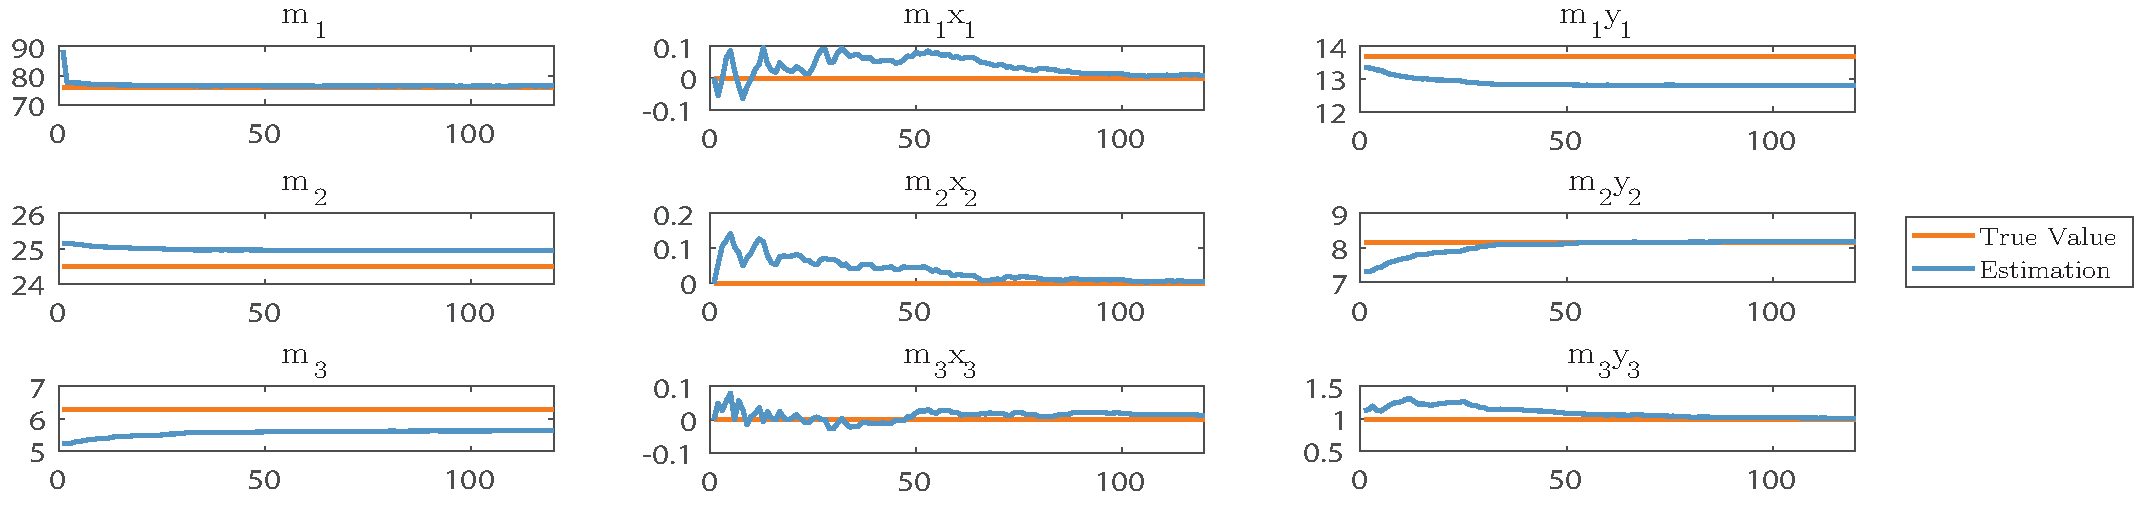
\includegraphics[width=0.9\linewidth]{figs/Value3_fixed2.pdf}
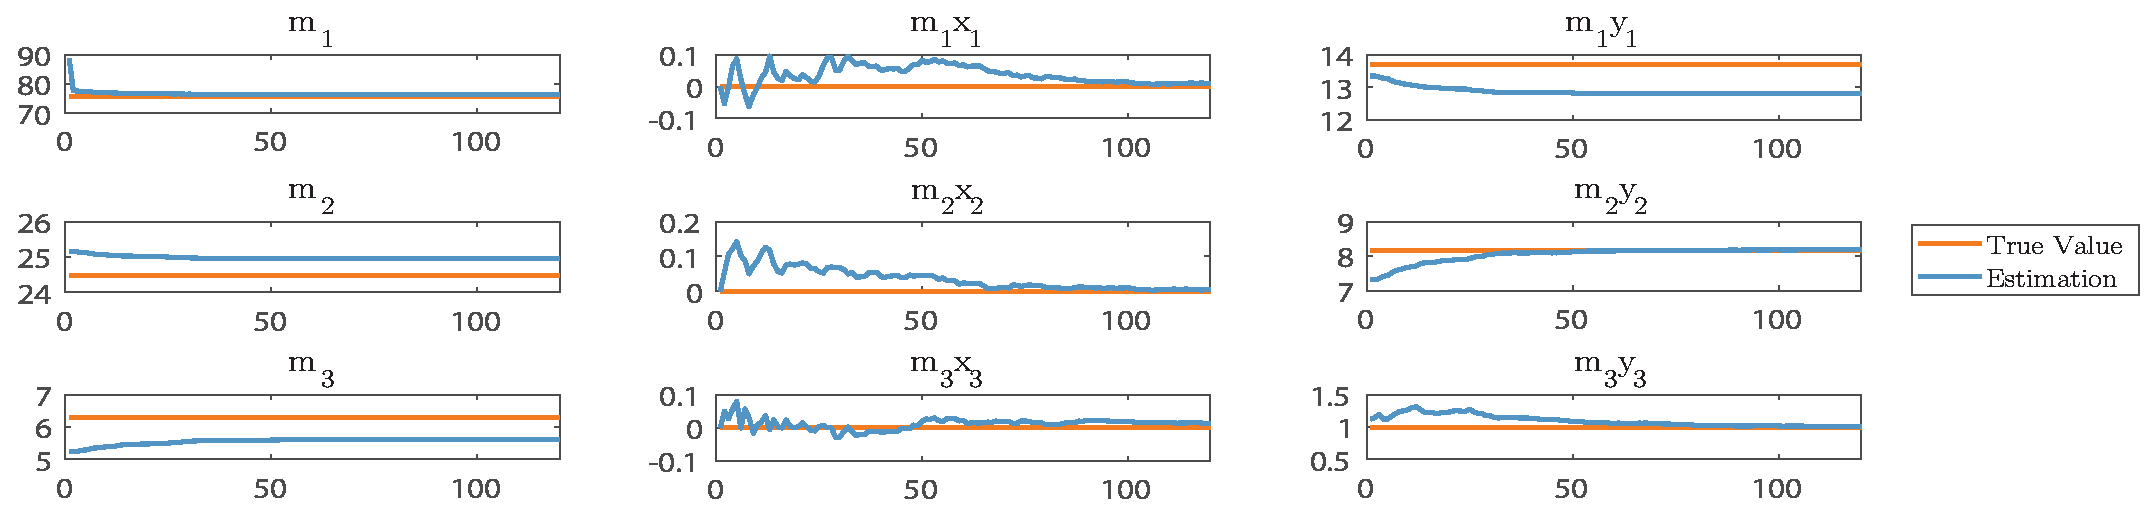
\includegraphics[width=0.9\linewidth]{figs/Value3_fixed2.eps}
\vspace{-.5\baselineskip}
\caption{\label{fig:Values} Values of the different parameters of the estimated model over 120 different configurations. The red lines show the real value of the parameter for the real robot, while the blue lines show the learned weights.}
\end{figure*}
To evaluate the performance of our algorithms we instantiated two full $L$-link \ac{WIP} models -- a ground truth model and an inaccurate model with an estimation of the parameters of the first robot. These two models served as placeholders for the arm's configuration and mass parameters. We then simplified these two models into their single link representation (Fig.~\ref{fig: system} - right). In Matlab, using an ODE45 integration loop, we simulated the system dynamics from the ground truth model and then calculated the control signals based on the estimated simplified model. In the \ac{DART} implementation, the dynamics were updated automatically by the simulator. We first started by tuning our \ac{ADRC}'s LQR gains to be able to control the estimated simplified model to the balance position of the ground truth model. During this process, we iteratively set both models to randomized joint angles on the configuration space. After tuning the controller and observer parameters for each joints configuration, the \ac{ADRC} would balance the systems to its true balance position, i.e. for a given configuration $q_2, q_3, \dots, q_L$, the \ac{ADRC} would find the value of $q_1$ that balanced the system.

\subsection{Gradient Descent Simulation}
\label{subsec:sim_results}

The offset given by the \ac{ADRC} for the estimated model was used in a gradient descent algorithm to update our estimated model parameters. Starting with the Matlab simulation, the estimated model was subject to initial noise for the initial estimation of $20\%$ from the real values of the parameters $m_i$, $m_ix_i$ and $m_iy_i$. Since each link had different properties (similar to our experimental robot), the noise perturbation differed; the first link has an approximated mass of $70 kg$  which gives a noise around $14kg$, while the third link has a mass of $6kg$ which give us a noise around $1.2kg$. Using \cref{eq:gradient_Descent} we update our $\beta$ for each iteration. A subset of the parameters of $\beta$ are shown in \cref{fig:Values}.

% The gradient descent algorithm was tested on a simulated system, which allowed us to compare an evolving mass model against ground truth values provided by the simulator.



% During this work, we started with a $7$ \ac{DoF} WIP simulation in Matlab.
% The system was subject to an initial noise for the initial estimation of $20\%$ from the real values of the parameters $m_i$, $M_{xi}$ and $M_{yi}$. Since each link had different properties, the noise perturbation differs, e.g. the first link has an approximated mass of $70 kg$  which gives a noise around $10kg$, while the third link has a mass of $6kg$ which give us a noise around $1kg$.
% For the experiments, given a configuration $q_2, q_3, \dots$, the disturbance rejection algorithm gives us the true value of $q_1$ to balance the robot.
% For this state vector $q$, we compute the $f(q)$ for our system and the gradient $\Delta$ for our $\beta$ update.
% As we update the parameters, the estimate of our $\beta$ changes over time. A subset of the parameters are shown in Fig.~\ref{fig:Values}.
It can be seen in \cref{fig:Values} that our algorithm modifies the $\beta$ vectors, reaching a local minimum. For some parameters (as $m_1$, $m_1y_2$ or $m_3y_3$) the estimated values converge to the real values, while for others (as $m_2$, $m_3$ or $m_1y_1$) the values converge to a constant error. Even though we are finding a local minima and not necessarily the correct values, we will show that our new estimate of $\beta$ improves upon the initial values. After running different simulations, we notice that while the system always reaches a $x_{CoM}$ error of zero, the weights converge to different values -- giving the intuition that the system consists of several local minima.

This method has shown that the approach works in finding a better set of values than the ones we initially started with, but might not get to the global optimum (the real values). We think that this happens because of the nonlinearities of the system and because the $\beta$ vector is not perfectly decoupled to the value of the masses.
% Over several simulations, different values of $\eta$ and $\mu$ were used, and the final values were set to $0.05$ and $0.1$ respectively.
% These values were chosen as they allow for fast convergence, which is a desired feature, as balancing the robot is not an easy task and we want to converge as quickly as possible \Bogdan{This sentence needs rewording}. If the learning rates \Bogdan{Both $\eta$ and $\mu$ or just $\eta$?} are increased, the gradient descent becomes unstable. Also, the results seem to be robust to noise, because a $20\%$ error in the initial estimation is considered big \Bogdan{considered big by whom. Give some reason like the robot fails to balance or something along these lines}.

\subsection{Meta-learning for Gradient Descent Convergence}
\label{subsec:Meta-learning}
As described in section \ref{subsec: meta-learning}, we simulated 20,000 poses over 500 erroneous $\beta$s, and got a set of 528 poses until the error was $2mm$. Without using the meta-learning algorithm this process takes  over 5,000 poses. The result of our simulated learning curve is presented in \cref{fig:Error_sim}. We tested for several initial erroneous $\beta$s which started with an $x_{CoM}$ error of at least $2 cm$ with a standard deviation of $0.5 cm$. It can be seen that after $500$ updates using the optimal poses, the mean error decreased to almost $0 cm$, specifically the max $\beta$ error decreased to $x_{tol} = 2mm$.
\begin{figure} [htb]
\centering
%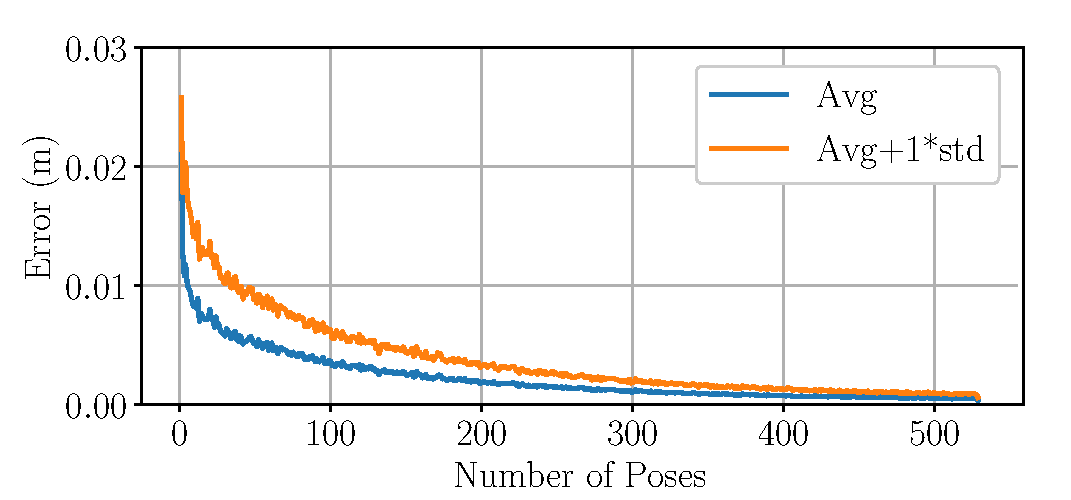
\includegraphics[width=0.8\columnwidth]{figs/Simulation_results.pdf}
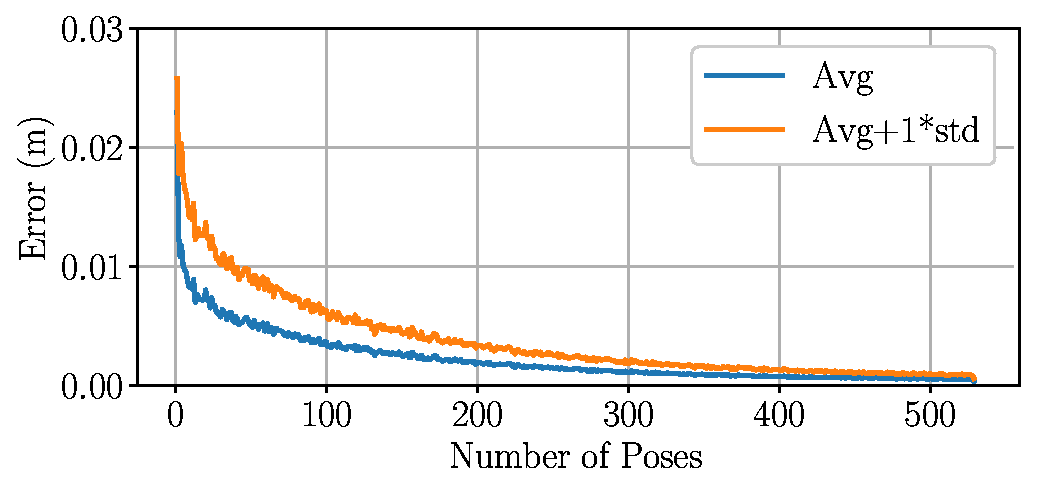
\includegraphics[width=0.8\columnwidth]{figs/Simulation_results.eps}
\vspace{-0.8\baselineskip}
\caption{\label{fig:Error_sim} Mean Error of several $\beta$s through the learning algorithm for the meta-learned best 500 poses.}
\end{figure}

% Even though the system is converging to a set of weights $\beta$ such that the value of $x_{CoM}$ is driven to $0$, it seems that the system is finding local optima and not converging to the true values. In Fig.~\ref{fig:Values} we can see how the different values of the systems change over time, to improve the estimation of the system. It can be noticed that some variables approach the real values, e.g. $m_1$ and $M_{y2}$ started with an error and converged to the real value, but other element's error increased or converged to a constant error.  After running different experiments, we notice that the systems always converges, but to different sets of weights, which gives the intuition that the system consists of several local minimas.



%To test the improvement of the parameter estimation of our robot, we implemented the stages of our algorithm in simulation and then implemented a offline version of the pipeline on the physical system.  We first developed our algorithm in a custom 2D simulation (Matlab), wherein we explicitly provided equations for the system dynamics.  We then implemented the same algorithm in a 3D dynamics simulator (DART) and then transition to the physical hardware of Golem Krang.

%%%%%%%%%%%%%%%%%%%%%%%%%%%%%%%%%%%%%%%%%%%%%%%%%%%%%%%%%%%%%%%%%%%%%%%%%%%%%%%%
% \subsection{Simulated System}
% \label{subsec:simulation}

% First, we implemented the balancing procedure in the 2D Matlab environment.  Our simulator provided the class methods for instantiating n-link \ac{WIP} models, updating their mass parameters, approximating their dynamics, applying control, and visualizing the results.  To test our robust controller, we instantiated two full n-link \ac{WIP} models--a ground truth model and our inaccurate initial estimate of this model. These two models served as placeholders, holding the current arm configuration and mass parameters.  We then simplified these two models into their single link representations.  Within an ODE45 integration loop, we both simulated the system dynamics and calculated the control signals. Our dynamics simulation had access to the simplified true model whereas our controller had access only to the simplified estimated model.

% To test our disturbance rejection, we initialized the arm links of our full ground truth model to randomized angles and masses.  We then copied these mass parameters (with noise) to our full approximate model. We controlled with knowledge of the simplified approximate model after simulating each time step with the true model.  We carefully tuned the controller and observer parameters to allow the system to balance.  The algorithm corrected center of mass angle offset for the simple approximate model, and we used this offset to correct the base angle of the full estimate model.  We iterated over different arm poses, forwarding each balanced pose as an input to the online learning algorithm.

% Once we had the pipeline working in simulation, we executed the meta-learning algorithm to get a set of the best poses to later acquire the data from the real robot.


% %%%%%%%%%%%%%%%%%%%%%%%%%%%%%%%%%%%%%%%%%%%%%%%%%%%%%%%%%%%%%%%%%%%%%%%%%%%%%%%%
% \subsection{Physcial System}
% \label{subsec:physical}

% Unlike our simulation environments which have omniscient knowledge of the world state, the physical hardware does not offer any easy method for determining the system's ground truth mass model. Thus, before implementing the entire online pipeline on the robot, we tested on the real system in an offline fashion. First, we manually set the robot to 190 poses given by the meta-learning algorithm. For each position we stabilized the system and then calculated the value of $x_{CoM}$ which the robot believes it has for the given $\beta_0$. After we acquired all this data on the Golem Krang, we performed the gradient descent algorithm to obtain the differents $\beta_i$. Finally, we tested some of these $\beta$s to show the performance of the robot. We picked the action of standing up, which is one of the most demanding action. For this action, the robot goes from a 3 contact point statically stable position to a balanced WIP position. Using a the same controller but different mass models for the each test, we compare the control input needed to make this action and then compare the state during the balance and how good the balance is.

%Without an easy method for determining the ground truth mass model of the physical hardware,

%Balance using joystick; record energy of controller

%%%%%%%%%%%%%%%%%%%%%%%%%%%%%%%%%%%%%%%%%%%%%%%%%%%%%%%%%%%%%%%%%%%%%%%%%%%%%%%%
%%%%%%%%%%%%%%%%%%%%%%%%%%%%%%%%%%%%%%%%%%%%%%%%%%%%%%%%%%%%%%%%%%%%%%%%%%%%%%%%
%%%%%%%%%%%%%%%%%%%%%%%%%%%%%%%%%%%%%%%%%%%%%%%%%%%%%%%%%%%%%%%%%%%%%%%%%%%%%%%%
\section{Experimental Results}
\label{subsec:results}

% \subsection{ADRC Simulation}
% The balancing of the robot using disturbance observers is presented in Fig.~\ref{fig:EDO_results}. The first graph shows the angle of the \ac{CoM} of both the real and the approximate model over time where it can be seen that the real system is heading towards 0 even though the approximate model is not. The other graphs show the wheel displacement as well as the input torque to the system.
% \begin{figure}[h]
% \centering
% 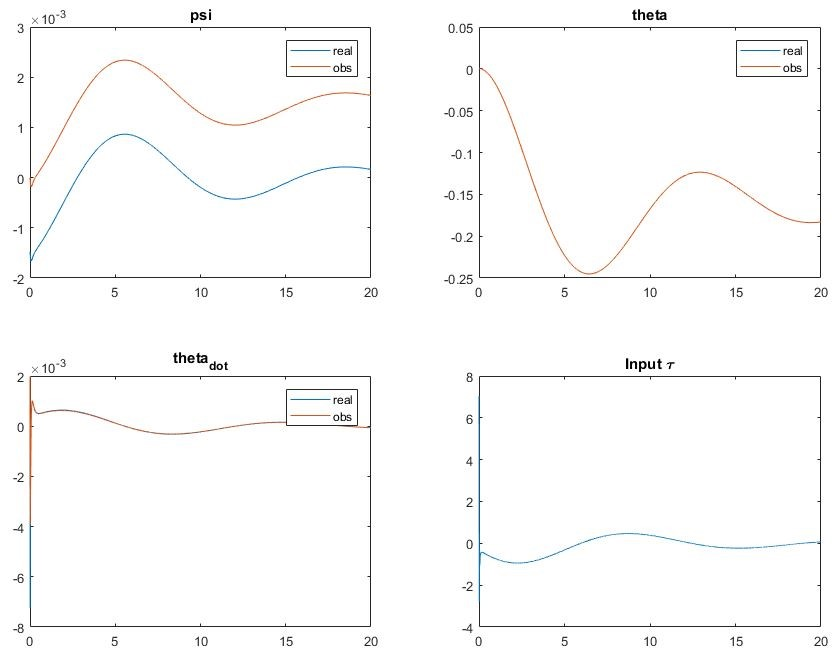
\includegraphics[width=0.99\columnwidth]{figs/EDO_results.jpg}
% \caption{\label{fig:EDO_results} Results of the State Observer Disturbance Rejection.\fixme{Make more descriptive caption}}
% \end{figure}
% We have that the difference between real system
%%%%%%%%%%%%%%%%%%%%%%%%%%%%%%%%%%%%%%%%%%%%%%%%%%%%%%%%%%%%%%%%%%%%%%%%%%%%%%%%





%%%%%%%%%%%%%%%%%%%%%%%%%%%%%%%%%%%%%%%%%%%%%%%%%%%%%%%%%%%%%%%%%%%%%%%%%%%%%%%%
% \subsection{Physical System Results}
% \label{subsec:phys_results}
% Unlike our simulation environments (in which we have an omniscient knowledge of the world state), actual hardware does not provide an easy method for determining the system's ground truth mass model.
For the robot that we are using, Golem Krang \cite{Stilman2010}, determining its mass model link-by-link is intractable.  Furthermore, the summarizing \ac{CoM} described in \ref{sec:method} is difficult to obtain.  Instead of extracting the full mass model or \ac{CoM} estimates, we follow the procedure of other work \cite{bature2014comparison,khosla2013performance} to evaluate balancing performance.  Where the authors analyze more readily observable phenomena, such as distance traveled, time spent stabilizing, and power consumption.  In our case, these quantities were used to analyze whether or not subsequent refinements of an initial offset estimation $(\beta_0)$ improves the stabilizing control.
The physical experiments were separated in two parts: manual data collection and controller efficiency testing.
% First, we manually set the robot to 230 poses given by the meta-learning algorithm. For each position we stabilized the system and then calculated the value of $x_{CoM}$ which the robot believes it has for the given $\beta_0$. After we acquired all this data on the Golem Krang, we performed the gradient descent algorithm to obtain the differents $\beta_i$. Finally, we tested some of these $\beta$s to show the performance of the robot. We picked the action of standing up, which is one of the most demanding action. For this action, the robot goes from a 3 contact point statically stable position to a balanced WIP position. Using a the same controller but different mass models for the each test, we compare the control input needed to make this action and then compare the state during the balance and how good the balance is.
For the first part, we collected data from our subset of pre-determined balanced poses -- we manually positioned the robot in the first 236 poses acquired from the meta-learning algorithm in \cref{subsec: meta-learning} and calculated the error between the real $x_{com}$ and the estimation.  We obtained this error by setting the robot to presumed balanced pose (which may not actually be balanced under our inaccurate $\beta_0$), and adjusted the base link angle $q_1$ until the system became balanced.  We then separated this data into a training set of 190 poses and a testing set of 46 poses.  Then, using the training set, we implemented gradient descent to obtain a series of betas going from $\beta_1, \beta_2, \dots, \beta_{190}$. For each beta, we computed the errors produced by the remaining balanced poses in the testing dataset; the results are shown in Fig.~\ref{fig:Error_hardware}.
\begin{figure}
\centering
%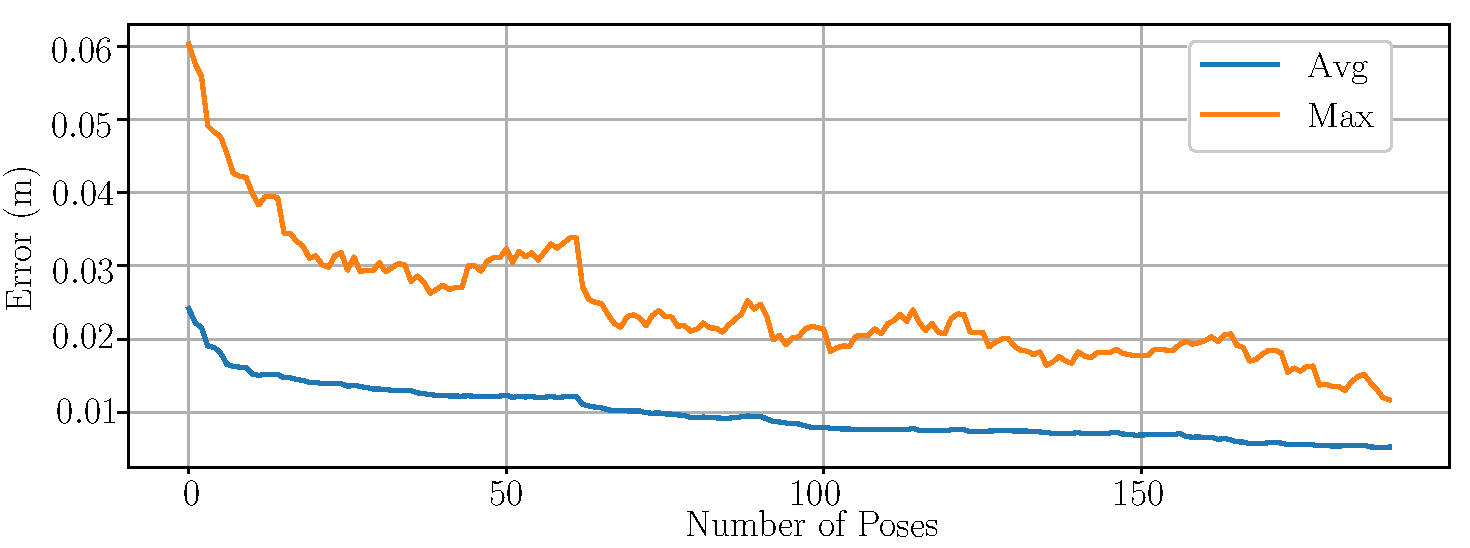
\includegraphics[width=0.9\columnwidth]{figs/TestingHardware.pdf}
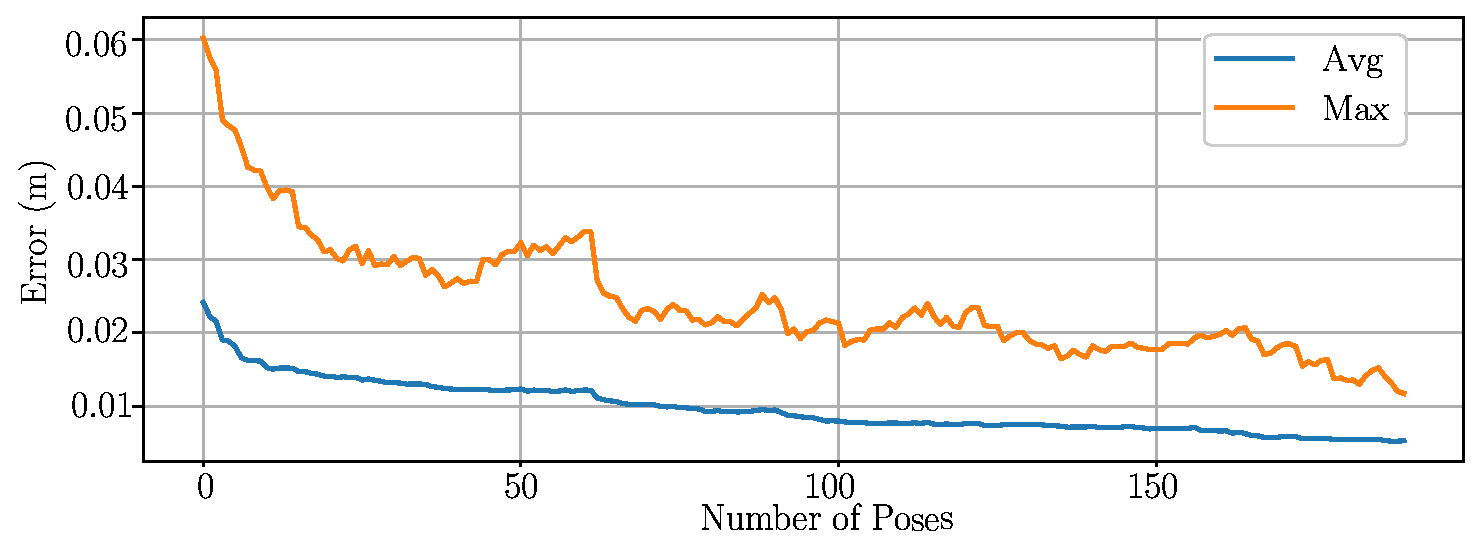
\includegraphics[width=0.9\columnwidth]{figs/TestingHardware.eps}
\vspace{-0.2cm}
\caption{\label{fig:Error_hardware} Error in the parameters as we update the weights $\beta$ for different random configurations.}
\end{figure}
For $\beta_0$, we started with a mean error of $2.5 cm$ in the $x_{CoM}$ for the given $46$ poses and a maximum error of $6 cm$. With subsequent iterations, the mean error and the maximum error decreased. For $\beta_{190}$ we achieved a mean error of $0.4 cm$ with a maximum error of $1.2 cm$ for any given pose in the testing set.

For the second part, we used five of our learned $\beta$s to balance the robot in a given pose.  Specifically, we looked at the initial balancing action, which involves transitioning between a stable sitting position to an inverted pendulum position. For this action, the robot stands from three points of contact with the ground (two active wheels and a caster wheel). Then it rotates its wheels (at a speed which depends on its \ac{CoM} estimate) to lift off the caster, and it finally balances as a two-wheeled \ac{WIP}.
The balancing experiments tested different $\beta$ estimates to show how the overall control improves during the transition and steady state of the robot.
% Based on the simulation results, we observed that the initial $\beta$ updates yielded the greatest improvement.
To investigate the connection between updated $\beta$ vectors and controller performance, we show the results of testing $\beta_{16}$, $\beta_{32}$, $\beta_{64}$, $\beta_{128}$ and $\beta_{190}$.  Smaller $\beta$s are not shown, since the robot controller was not able to securely stabilize the system.  Additionally, for each $\beta_i$ we tested seven attempts to see the reproducibility of the results.

The instantaneous power consumption of the wheel motors during and after the transition to standing is shown in \cref{fig:betas_comparison}, and a summary of the control performance is presented in Table~\ref{tab:control_performance}.  The instantaneous power was calculated by multiplying the torque and angular velocity of the wheels.

\begin{figure}[h]
\centering
% 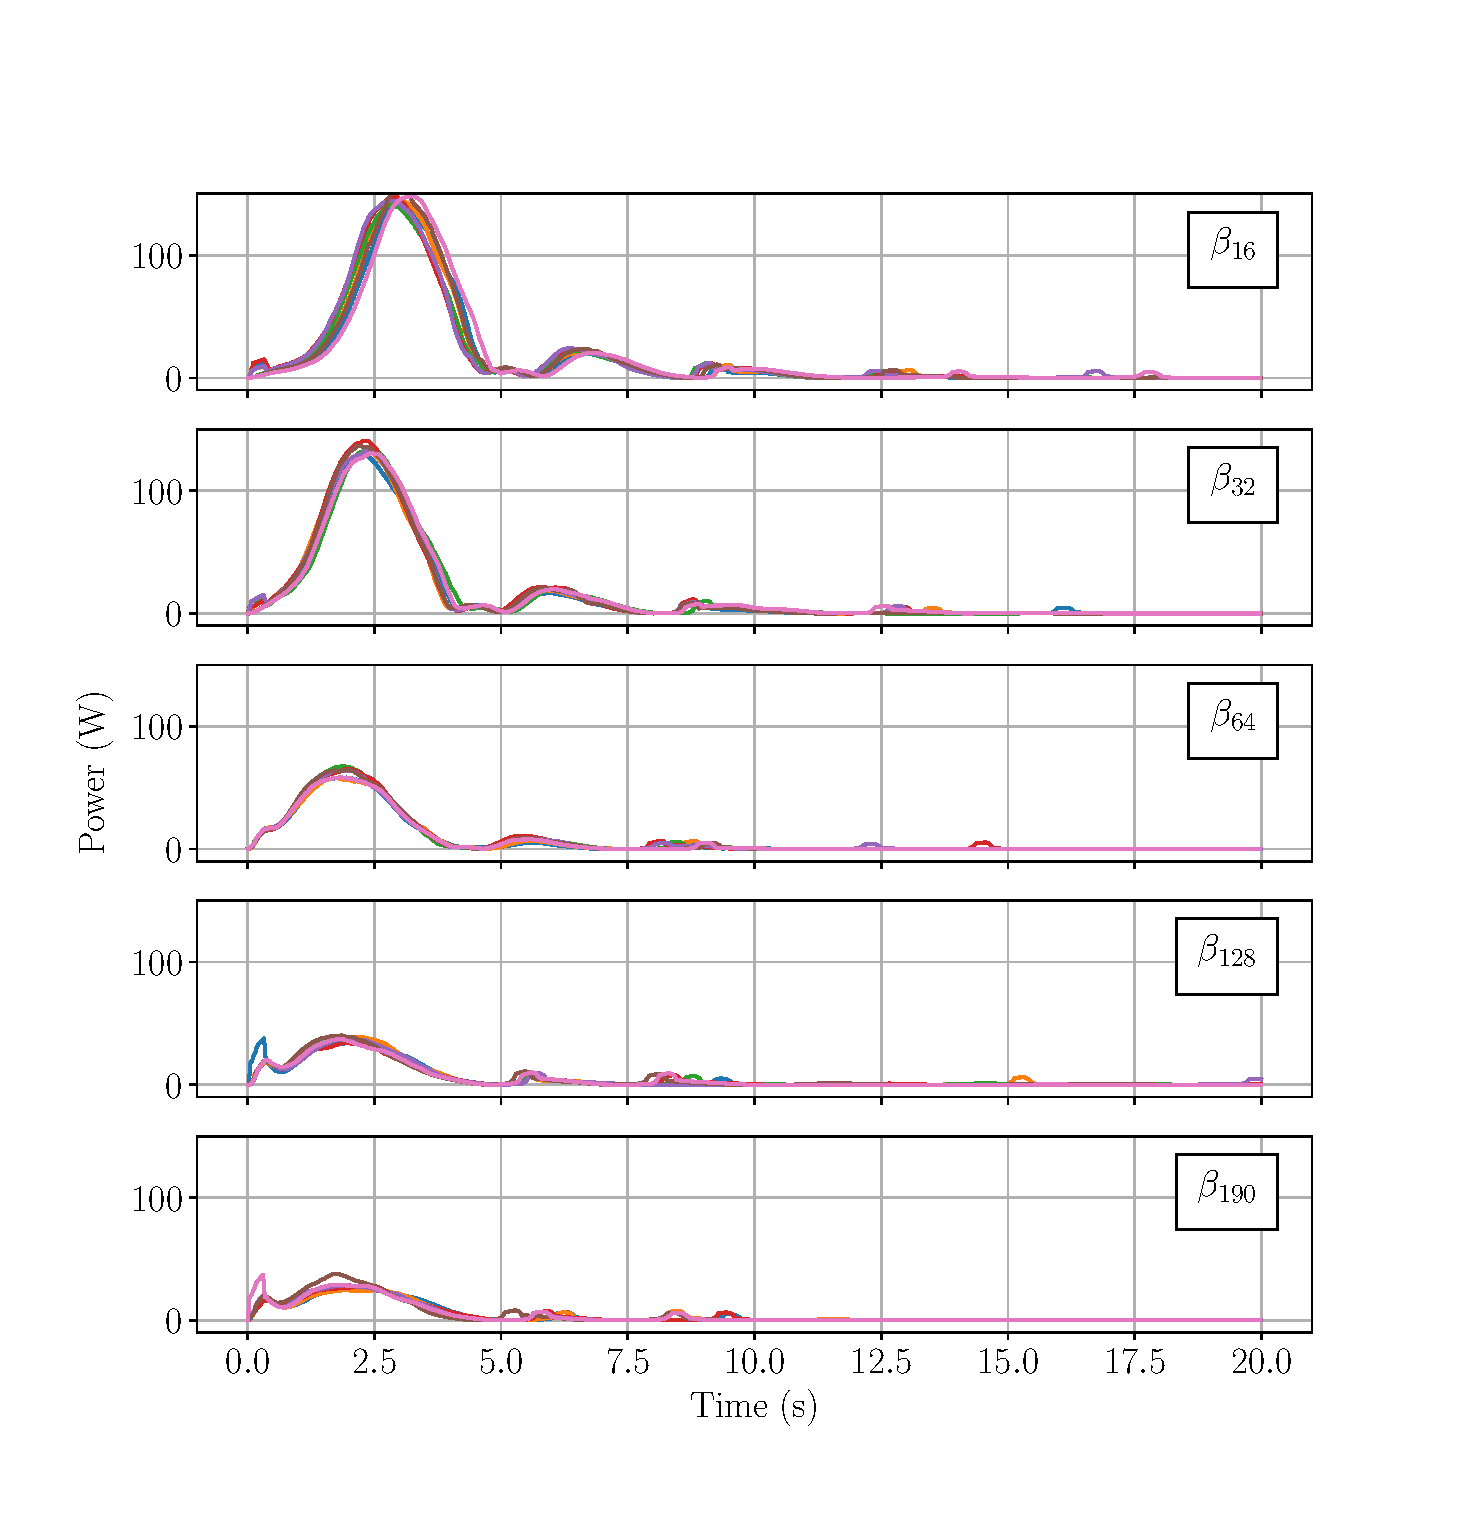
\includegraphics[width = 0.99\columnwidth]{figs/Power_20s.eps}
% 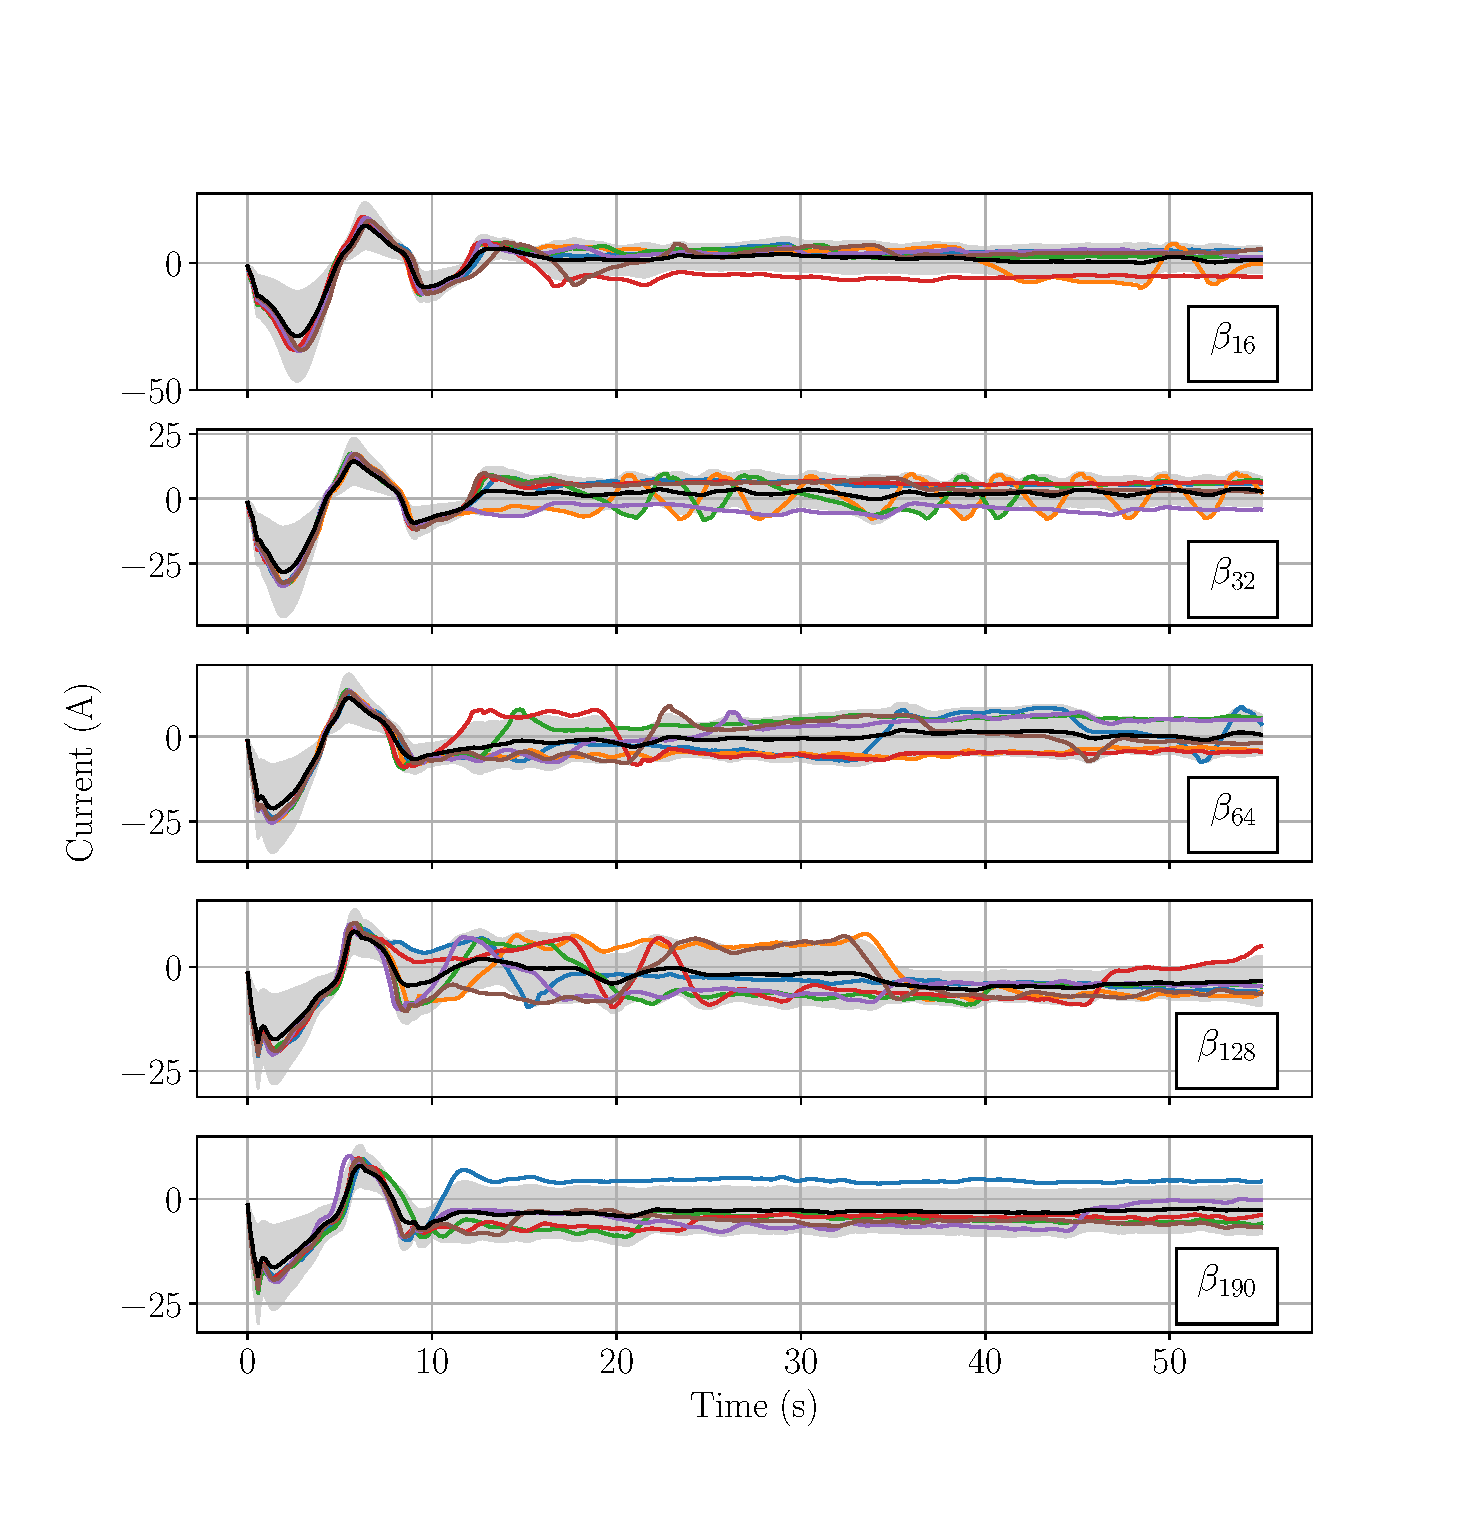
\includegraphics[width = 0.99\columnwidth]{figs/currentAveragesBetas.eps}
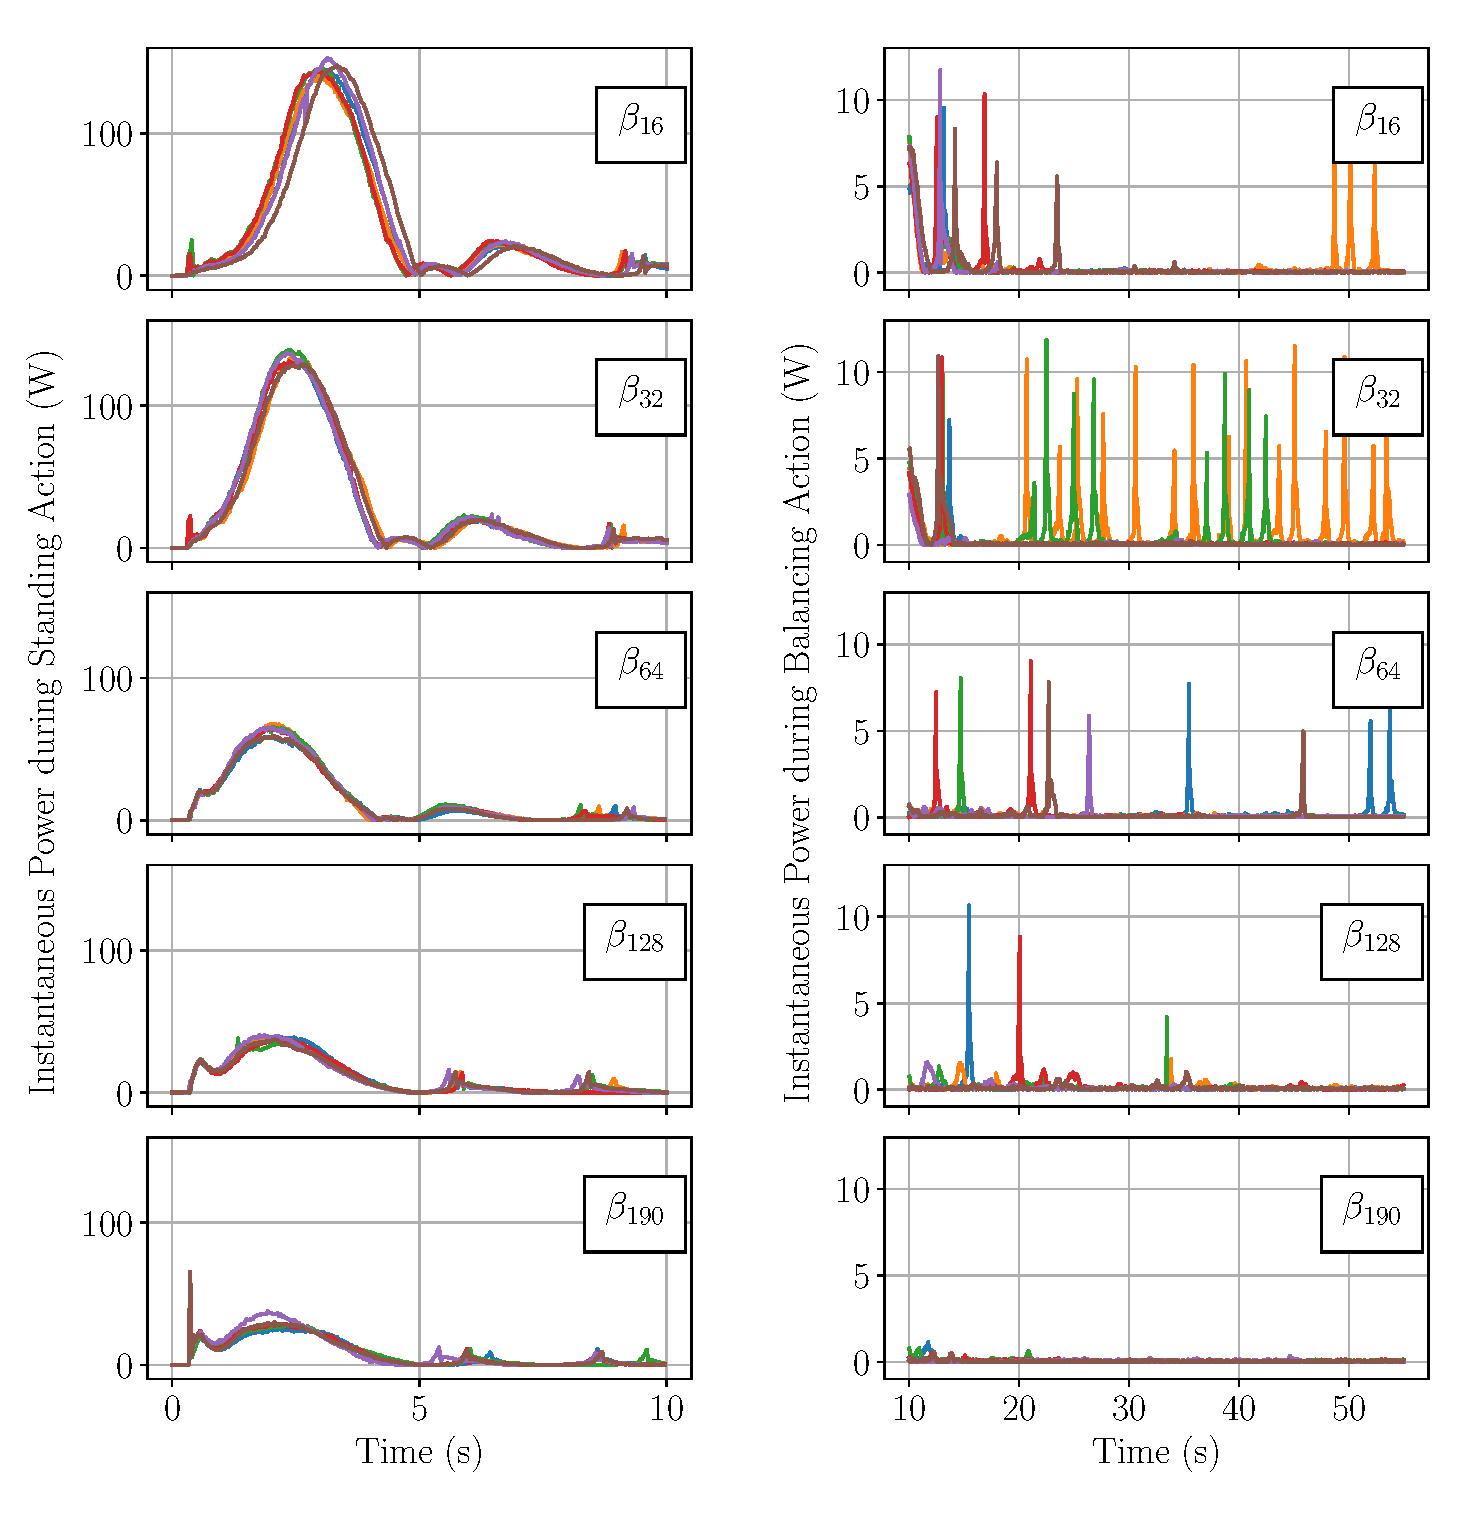
\includegraphics[width = 0.99\columnwidth]{figs/dualColumn.eps}
% 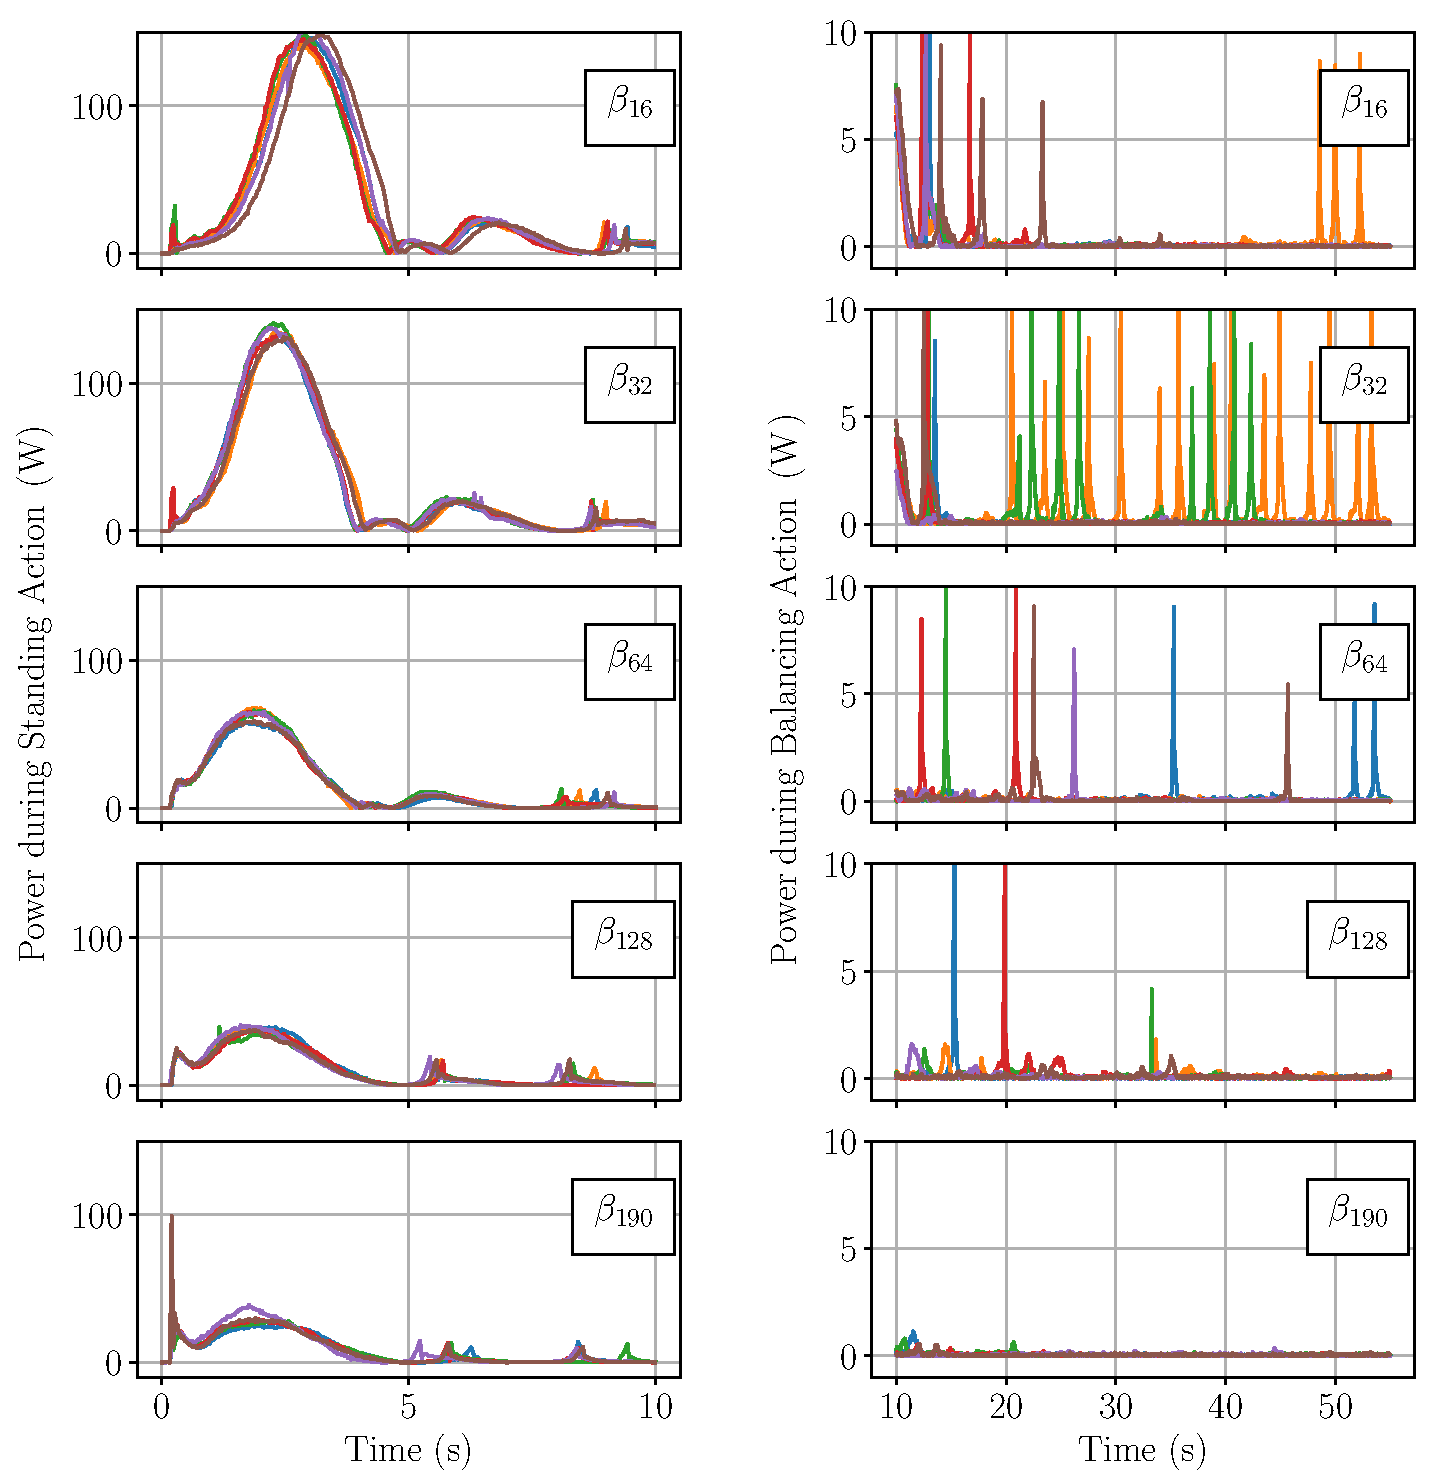
\includegraphics[width = 0.99\columnwidth]{figs/Power.pdf}
\vspace{-1.5\baselineskip}
\caption{\label{fig:betas_comparison} Instantaneous power applied by the wheel motors.  Each plot includes the results corresponding to 7 independent runs for different values of $\beta$ ($\beta_{16}$, $\beta_{32}$, $\beta_{64}$, $\beta_{128}$ and $\beta_{190}$). The left column summarizes the sitting-standing transition (the first 10 seconds of the experiment), and the right column summarizes the \ac{WIP} balancing (the subsequent 10 to 60 seconds).}
\end{figure}

\begin{table}[h!]
% \begin{table*}[t]
\centering
\caption{\label{tab:control_performance} Summary of the control performance under different betas.}
\vspace{-\baselineskip}
\begin{tabular}{c|p{0.9cm}|p{1.0cm}|p{1.4cm}|p{1.0cm}|p{1.5cm}}
% \begin{tabular}[width=\linewidth]{c|c|c|c|c|c}
$\beta$ & Max Pos. [m] & Resting Pos. [m] & Time until Resting [s] & Max Power [W] & Avg. Resting Power [mW] \\
\hline
\hline
$\beta_{16}$ &  $4.70 \pm 0.16$ & $2.49 \pm 0.03$ & $11.5 \pm 1.5$  &  $145 \pm 4$ & $7.83 \pm 1.69$\\
\hline
$\beta_{32}$ & $4.59 \pm 0.11$ & $2.67 \pm 0.11$ & $10.1 \pm 1.1$  &  $133 \pm 4$ & $8.85 \pm 7.09$\\
\hline
$\beta_{64}$ & $3.59 \pm 0.17$ & $1.53 \pm 0.05$ & $7.59 \pm 1.33$  &  $63.1 \pm 3.3$ & $2.95 \pm 1.04$\\
\hline
$\beta_{128}$ & $2.74 \pm 0.07$ & $1.13 \pm 0.03$ & $6.80 \pm 1.20$  &  $41.3 \pm 6.9$ & $2.90 \pm 0.60$\\
\hline
$\beta_{190}$ & $\bf 2.61 \pm 0.08$ & $\bf 1.08 \pm 0.03$ & $\bf 7.09 \pm 1.97$  & $\bf 34.5 \pm 13.2$ & $\bf 1.54 \pm 0.25$ \\
\end{tabular}
% \end{table*}
\end{table}

% \begin{table}[h!]
% %\begin{table*}[h!]
% \centering
% \caption{\label{tab:control_performance} Summary of the control performance under different betas.}
% \begin{tabular}{c|p{1.0cm}|p{1.0cm}|p{1.4cm}|p{0.9cm}|p{1.4cm}}
% %\begin{tabular}[width=\linewidth]{c|c|c|c|c|c}
% $\beta$ & Peak Pos. [m] & Resting Pos. [m] & Time until Resting [s] & Peak Power [W] & Avg. Resting Power [W] \\
% \hline
% \hline
% $\beta_{16}$ & $4.70 \pm 0.16$ & $2.49 \pm 0.03$ & $11.5 \pm 1.5$  &  $145 \pm 4$ & $0.00783 \pm 0.00169$\\
% \hline
% $\beta_{32}$ & $4.59 \pm 0.11$ & $2.67 \pm 0.11$ & $10.1 \pm 1.1$  &  $133 \pm 4$ & $0.00885 \pm 0.00709$\\
% \hline
% $\beta_{64}$ & $3.59 \pm 0.17$ & $1.53 \pm 0.05$ & $7.59 \pm 1.33$  &  $63.1 \pm 3.3$ & $0.00295 \pm 0.00104$\\
% \hline
% $\beta_{128}$ & $2.74 \pm 0.07$ & $1.13 \pm 0.03$ & $6.80 \pm 1.20$  &  $41.3 \pm 6.9$ & $0.00290 \pm 0.00060$\\
% \hline
% $\beta_{190}$ & $\bf 2.61 \pm 0.08$ & $\bf 1.08 \pm 0.03$ & $\bf 7.09 \pm 1.97$  & $\bf 34.5 \pm 13.2$ & $\bf 0.00154 \pm 0.00025$ \\
% \end{tabular}
% %\end{table*}
% \end{table}

As shown in the left column of Fig.~\ref{fig:betas_comparison} and in Table~\ref{tab:control_performance}, the peak power consumption decreases with subsequent values of beta.  As shown in the right column of the same figure, the number of balancing adjustments (spikes in power consumption) is similarly reduced.  For the first $\beta$ values, the system occasionally destabilized and readjusted, whereas the latest $\beta_{190}$ value kept these adjustments and hence overall power consumption to a minimum.

Table~\ref{tab:control_performance} shows improvement in several quantities that characterize control performance: the initial overshoot position decreases by $44\%$ between the $\beta_{16}$ and $\beta_{190}$ iterations; the resting position decreases by $57\%$; the time until resting decreases by $38\%$; the peak instantaneous power decreases by $76\%$; and the average power during steady state balancing decreases by $80\%$.  Each of our performance metrics improves with more refined mass model parameters.  Together, these trends support the claim that the \ac{CoM} estimation procedure does improve balancing for a \ac{WIP}.

% Our $\beta$ parameters reduced the table~\ref{tab:control_performance} column quantities of the initial $\beta_{16}$ parameters by $44\%$, $57\%$, $38\%$, $76\%$, $80\%$, respectively.

%%%%%%%%%%%%%%%%%%%%%%%%%%%%%%%%%%%%%%%%%%%%%%%%%%%%%%%%%%%%%%%%%%%%%%%%%%%%%%%%
%%%%%%%%%%%%%%%%%%%%%%%%%%%%%%%%%%%%%%%%%%%%%%%%%%%%%%%%%%%%%%%%%%%%%%%%%%%%%%%%
%%%%%%%%%%%%%%%%%%%%%%%%%%%%%%%%%%%%%%%%%%%%%%%%%%%%%%%%%%%%%%%%%%%%%%%%%%%%%%%%
\section{Conclusion}
\label{sec:conclusion}
We have shown that the proposed methodology improves the \ac{CoM} estimate of a \ac{WIP} Humanoid and that these improvements translate to improved controller performance.
In simulation, using active disturbance rejection control, our robot successfully balances with an inaccurate prior mass model, collects new pose data at balanced positions, and learns from these poses to produce a more accurate \ac{CoM} estimate.
In hardware, we demonstrate that these refined estimates directly translate into improved controller performance.
Together, our simulation and hardware results support the claim that our algorithm -- a semi-automated, tractable procedure that refines the latent space mass model of a high dimensional system with few physically observable parameters -- does improve overall balance.  The algorithm was probed in simulation and verified physically on a 19 \ac{DoF} \ac{WIP} robot.
Our future work will implement the fully automated estimation pipeline--active disturbance rejection control, balanced pose data collection, and online learning--in an entirely online fashion on the physical robot, where it will improve its parameter estimates through meta-learned poses.

%%%%%%%%%%%%%%%%%%%%%%%%%%%%%%%%%%%%%%%%%%%%%%%%%%%%%%%%%%%%%%%%%%%%%%%%%%%%%%%%
%%%%%%%%%%%%%%%%%%%%%%%%%%%%%%%%%%%%%%%%%%%%%%%%%%%%%%%%%%%%%%%%%%%%%%%%%%%%%%%%
%%%%%%%%%%%%%%%%%%%%%%%%%%%%%%%%%%%%%%%%%%%%%%%%%%%%%%%%%%%%%%%%%%%%%%%%%%%%%%%%
% \section{Future Work}
% \label{sec:future}

% \fixme{TODO: Munzir, Talk about Krang Full Body Control}

% On the online learning side, there are also many paths to follow for future progress. The current gradient descent still requires hundreds of examples to train on so developing a method to provide more information rich examples could greatly reduce the training time. There is also more work that could be done on the gradient descent algorithm to allow it converge faster such as adaptive learning rates. In general, the gradient descent seems to get stuck in local minima for the parameters. Because of this, implementing a different learning algorithm could also lead to better results. Potential options are simulated annealing and stochastic gradient descent to converge to the true minima instead of a local minima.

\bibliographystyle{IEEEtran}
\bibliography{IEEEabrv,onlinecom}
\end{document}
